% Compliance-as-Code AI Auditor -- Advanced Machine Learning report (UBB Cluj, 2026-2027).
% Adapted from the course template (lauradiosan/AML-MateInfoUBB, 2026-2027/Report/texModel/model.tex).
% Build: `make` (uses tectonic) or `latexmk -pdf report.tex`. See Makefile.

\documentclass[a4paper,11pt]{report}

\usepackage{algorithmic}
\usepackage{algorithm}
\usepackage{array}
\usepackage{amsmath}
\usepackage{amsfonts}
\usepackage{amssymb}
\usepackage{amsthm}
\usepackage{booktabs}
\usepackage{caption}
\usepackage{comment}
\usepackage{enumitem}
\usepackage{fancyhdr}
\usepackage{iftex}
\ifPDFTeX
  \usepackage[T1]{fontenc}
  \usepackage[utf8]{inputenc}
\fi
\usepackage{lmodern}
\usepackage{geometry}
\usepackage{graphicx}
\usepackage{multicol}
\usepackage{multirow}
\usepackage{pgfgantt}
\usepackage{setspace}
\usepackage{tabularx}
\usepackage{tikz}
\usetikzlibrary{arrows.meta,positioning,shapes.geometric,shapes.multipart,fit,backgrounds,calc}
\usepackage{url}
\usepackage{verbatim}
\usepackage{xcolor}
\usepackage[numbers,sort&compress]{natbib}
\usepackage[colorlinks]{hyperref}

\geometry{a4paper,top=3cm,left=2cm,right=2cm,bottom=3cm}

% ------------------------------------------------------------------ placeholders (render in red)
\newcommand{\todo}[1]{\textcolor{red}{\textbf{[TODO: #1]}}}
% Marks a number / table / figure that the experiments run must still fill in.
\newcommand{\resultsTODO}[1]{\par\noindent\fcolorbox{red}{red!5}{\parbox{\dimexpr\linewidth-2\fboxsep-2\fboxrule\relax}{\small\textcolor{red}{\textbf{RESULTS PENDING:} #1}}}\par}
% Inline numeric placeholder, e.g. accuracy \res{acc-hybrid}.
\newcommand{\res}[1]{\textcolor{red}{\textbf{[#1]}}}

% Includes figures/<name>.pdf or .png if the experiments agent produced it, otherwise a red placeholder.
\newcommand{\maybefig}[3][0.85\linewidth]{%
  \IfFileExists{figures/#2.pdf}{\includegraphics[width=#1]{figures/#2.pdf}}{%
  \IfFileExists{figures/#2.png}{\includegraphics[width=#1]{figures/#2.png}}{%
  \resultsTODO{figure \texttt{figures/\detokenize{#2}.\{pdf,png\}} not generated yet. #3}}}}

% ---------------------------------------------------------------------------
% Team identification. EVERY \todo{...} below renders in red in the PDF.
% Fill these in, then rebuild with `make` (see Makefile).
% ---------------------------------------------------------------------------
\newcommand{\BalcName}{B\^alc Felicia}
\newcommand{\BalcSpec}{\todo{specialisation}}
\newcommand{\BalcGroup}{\todo{group}}
\newcommand{\BalcEmail}{\todo{email}}

\newcommand{\DraghiciName}{Dr\u{a}ghici Eduard}
\newcommand{\DraghiciSpec}{\todo{specialisation}}
\newcommand{\DraghiciGroup}{\todo{group}}
\newcommand{\DraghiciEmail}{\todo{email}}

\newcommand{\GogName}{Gog Raluca}
\newcommand{\GogSpec}{\todo{specialisation}}
\newcommand{\GogGroup}{\todo{group}}
\newcommand{\GogEmail}{\todo{email}}

% Short author line used in the page header.
\newcommand{\AuthorsShort}{B\^alc, Dr\u{a}ghici, Gog}


\newcommand{\ProjectTitle}{Compliance-as-Code AI Auditor: Checking Applications Against Policies and Regulations (e.g., EU AI Act)}
\newcommand{\ProjectShort}{Compliance-as-Code AI Auditor}

% math shorthands
\newcommand{\St}{\mathcal{S}}
\newcommand{\Ev}{\mathcal{E}}
\newcommand{\Req}{\mathcal{R}}
\newcommand{\Cl}{\mathcal{C}}
\newcommand{\Lv}{\mathcal{L}}
\newcommand{\stat}[1]{\textsc{#1}}

\pagestyle{fancy}
\fancyhf{}
\fancyhead[R]{\ProjectShort}
\fancyhead[L]{\AuthorsShort}
\fancyfoot[L]{Advanced Machine Learning --- 2026-2027}
\fancyfoot[R]{\thepage}
\setlength{\headheight}{14pt}

\renewcommand{\headrulewidth}{2pt}
\renewcommand{\footrulewidth}{1pt}
\renewcommand{\headrule}{\hbox to\headwidth{%
  \color{lime}\leaders\hrule height \headrulewidth\hfill}}
\renewcommand{\footrule}{\hbox to\headwidth{%
  \color{lime}\leaders\hrule height \footrulewidth\hfill}}
\fancypagestyle{plain}{\fancyhf{}\fancyhead[R]{\ProjectShort}\fancyhead[L]{\AuthorsShort}%
  \fancyfoot[L]{Advanced Machine Learning --- 2026-2027}\fancyfoot[R]{\thepage}}

\hypersetup{
pdftitle={Compliance-as-Code AI Auditor},
pdfauthor={Balc Felicia, Draghici Eduard, Gog Raluca},
pdfkeywords={compliance-as-code, EU AI Act, GDPR, LLM-as-a-judge, retrieval-augmented generation, auditing},
bookmarksnumbered,
pdfstartview={FitH},
urlcolor=cyan,
colorlinks=true,
linkcolor=blue!60!black,
citecolor=green!50!black,
}

\setcounter{secnumdepth}{3}
\setcounter{tocdepth}{2}
\linespread{1}
\setlength{\emergencystretch}{3em}
\sloppy

\begin{document}

% ======================================================================= title page
\begin{titlepage}
\sloppy
\begin{center}

\includegraphics[width=2.2cm]{img/ubb.pdf}\\[0.4cm]
BABE\c S-BOLYAI UNIVERSITY, CLUJ-NAPOCA, ROM\^ANIA

FACULTY OF MATHEMATICS AND COMPUTER SCIENCE

\vspace{4.5cm}

{\LARGE \textbf{Compliance-as-Code AI Auditor}}\\[0.4cm]
{\Large Checking Applications Against Policies and Regulations (e.g., EU AI Act)}

\vspace{1cm}

\normalsize -- Advanced Machine Learning report --
\end{center}

\vspace{4cm}

\begin{flushright}
\Large{\textbf{Authors}}\\[0.2cm]
\normalsize
\BalcName, \BalcSpec, \BalcGroup, \BalcEmail\\
\DraghiciName, \DraghiciSpec, \DraghiciGroup, \DraghiciEmail\\
\GogName, \GogSpec, \GogGroup, \GogEmail
\end{flushright}

\vfill

\begin{center}
2026-2027
\end{center}
\end{titlepage}

\pagenumbering{gobble}

% Graphical abstract (TikZ). Used in the abstract (scaled) and in Chapter 2 (Figure~\ref{fig:graphical-abstract}).
% Note: inside \newcommand, TikZ style parameters must be written ##1.
\newcommand{\graphicalabstract}{%
\begin{tikzpicture}[
  font=\sffamily\footnotesize,
  box/.style={draw, rounded corners=2pt, align=center, minimum height=1.35cm, text width=2.75cm, inner sep=3pt, fill=##1},
  arr/.style={-{Stealth[length=2.2mm]}, thick},
  lab/.style={font=\sffamily\scriptsize, text=black!65, align=center}]

  % lanes
  \node[box=blue!8]   (pol)  at (0,2.2)   {\textbf{Policy} $P$\\EU AI Act, GDPR,\\internal policy};
  \node[box=blue!8]   (cl)   at (4.0,2.2) {\textbf{Clauses} $\Cl$\\citable ids\\\texttt{Art.12(1)}};
  \node[box=blue!8]   (req)  at (8.0,2.2) {\textbf{Requirements} $\Req$\\statement, tiers,\\checks, queries};
  \node[box=orange!10] (repo) at (0,0)     {\textbf{Repository} $D$\\code, IaC, config,\\docs, model cards};
  \node[box=orange!10] (ev)   at (4.0,0)   {\textbf{Evidence} $\Ev$\\line chunks\\+ signals};
  \node[box=orange!10] (risk) at (8.0,0)   {\textbf{Risk tier} $\rho$\\Art.~5 / Annex III /\\Art.~50};

  % evaluation
  \node[box=green!10]  (rules) at (12.0,2.2) {\textbf{Rule engine}\\regex, file, YAML,\\Rego checks};
  \node[box=violet!10] (judge) at (12.0,0)   {\textbf{LLM judge}\\Claude (headless)\\must cite evidence};
  \node[box=red!8]     (ver)   at (15.8,1.1) {\textbf{Verifier}\\citations exist\\and support claim};
  \node[box=yellow!20] (hitl)  at (19.6,1.1) {\textbf{Human gate}\\conflict or low\\confidence $\to$ review};
  \node[box=gray!10]   (rep)   at (23.4,1.1) {\textbf{Audit report}\\status, confidence,\\\texttt{file:line}, gaps,\\fixes; SARIF, UI};
  \node[draw, circle, fill=yellow!35, inner sep=1.5pt, font=\sffamily\scriptsize, align=center] (human) at (19.6,3.0) {human\\auditor};

  \draw[arr] (pol) -- node[lab, above]{ingest} (cl);
  \draw[arr] (cl) -- node[lab, above]{decompose} (req);
  \draw[arr] (repo) -- node[lab, above]{collect} (ev);
  \draw[arr] (ev) -- node[lab, above]{classify} (risk);
  \draw[arr] (req) -- node[lab, above]{evaluate} (rules);
  \draw[arr] (risk) -- node[lab, above]{applicable} (judge);
  \draw[arr, dashed] (rules) -- node[lab, right, xshift=1mm]{inconclusive\\or weak} (judge);
  \draw[arr] (ev.south) -- ++(0,-0.45) -| node[lab, below, pos=0.25]{BM25 retrieval of evidence for each requirement} (judge.south);
  \draw[arr] (rules.east) -- (ver.north west);
  \draw[arr] (judge.east) -- (ver.south west);
  \draw[arr] (ver) -- (hitl);
  \draw[arr] (hitl) -- (rep);
  \draw[arr, dashed] (human) -- node[lab, right]{decide /\\contest} (hitl);
\end{tikzpicture}}


\begin{abstract}
\noindent
\textbf{Relevance.} The EU Artificial Intelligence Act~\cite{euaiact2024} turns ethical principles into legally binding,
risk-tiered obligations (risk management, record-keeping, transparency, human oversight, robustness), which come on top of
GDPR~\cite{gdpr2016} and internal responsible-AI policies. Checking an application against these texts is today a manual,
document-heavy activity that is repeated whenever the code or the regulation changes.

\medskip\noindent
\textbf{Method.} We build a \emph{Compliance-as-Code AI Auditor}: policies are parsed into citable clauses and decomposed
into atomic, testable requirements (curated YAML or an LLM \emph{PolicyAnalyst} agent); an application repository is turned
into an index of evidence chunks (code, configuration, infrastructure-as-code, documentation, model cards, logs). Each
requirement is evaluated by a \emph{hybrid} orchestrator: a deterministic rule engine (regex, file, YAML-path and Rego checks)
runs first; inconclusive or weak cases are sent to an LLM \emph{ComplianceJudge} (Claude, invoked through the Claude Code CLI in
headless mode) that receives BM25-retrieved evidence and must cite it; a \emph{Verifier} removes hallucinated citations and
refuses ``compliant'' claims without evidence; disagreements and low-confidence verdicts are escalated to a human reviewer.
The output is an auditable report linking every requirement to \texttt{file:line} evidence or to a gap, with a risk tier,
a scorecard, remediation advice and SARIF output for CI.

\medskip\noindent
\textbf{Data.} Three policy corpora (selected EU AI Act provisions, GDPR, a fictional internal policy; 45 curated
requirements) and a benchmark of five hand-labelled AI application repositories (225 requirement-level labels) designed with
deliberate traps for rule-based checks (indirect evidence, decoys, requirements without rules).

\medskip\noindent
\textbf{Results.} \resultsTODO{one or two sentences with the headline numbers: accuracy / macro-F1 / false-compliance rate of
deterministic vs LLM vs hybrid, share of requirements routed to the LLM, citation validity, cost and latency per audit.}

\medskip\noindent
\textbf{Graphical abstract.}

\begin{center}
\resizebox{\linewidth}{!}{\graphicalabstract}
\end{center}
\end{abstract}


\tableofcontents
\newpage
\listoftables
\listoffigures
\listofalgorithms
\newpage

\setstretch{1.15}
\pagenumbering{arabic}

\chapter{Project and team}
\label{chapter:team}

\section{Project}
\textbf{Title:} \ProjectTitle. \textbf{Course:} Advanced Machine Learning, Faculty of Mathematics and Computer Science,
Babe\c s-Bolyai University, 2026-2027 (topic \#5). \textbf{Repository layout:} \texttt{app/backend} (Python package
\texttt{ccauditor}: engine, agents, CLI, REST API), \texttt{app/web} (Next.js dashboard), \texttt{app/benchmark}
(labelled target applications), \texttt{docs/} (design and this report).

\section{Team members, skills and roles}

Table~\ref{tab:team} identifies the team.

\begin{table}[htbp]
\caption{Team members, skills and roles.}
\label{tab:team}
\centering\small
\begin{tabularx}{\linewidth}{@{}p{2.6cm}p{3.6cm}X@{}}
\toprule
\textbf{Member} & \textbf{Identification} & \textbf{Skills and role} \\
\midrule
\BalcName & \BalcSpec, \BalcGroup \newline \BalcEmail &
\emph{Policy \& governance lead.} Regulatory analysis (EU AI Act, GDPR), policy corpus in citable markdown, curated
requirements YAML (statements, applicability, checks), benchmark labelling protocol, governance and ethics chapters. \\
\DraghiciName & \DraghiciSpec, \DraghiciGroup \newline \DraghiciEmail &
\emph{Architecture \& LLM lead.} Data contracts, orchestrator (deterministic / LLM / hybrid), Claude Code headless backend
with caching, agents (PolicyAnalyst, RiskClassifier, ComplianceJudge, Verifier, Remediator), CI integration. \\
\GogName & \GogSpec, \GogGroup \newline \GogEmail &
\emph{Evidence, UI \& evaluation lead.} Evidence collectors and BM25 retriever, web dashboard (traceability, review queue),
benchmark applications, experiment harness, metrics and figures. \\
\bottomrule
\end{tabularx}
\end{table}

\section{Performed tasks and timeline}

All members took part in the literature review, the weekly design reviews, the report and the presentation.
Figure~\ref{fig:gantt} shows the task plan over the 14 weeks of the semester.

\begin{figure}[htbp]
\centering
\resizebox{\linewidth}{!}{%
\begin{ganttchart}[
  hgrid, vgrid={*1{black!15,dotted}},
  x unit=0.75cm, y unit chart=0.55cm,
  bar/.append style={fill=blue!30},
  group/.append style={fill=black!60},
  milestone/.append style={fill=red!70},
  bar label font=\small, group label font=\small\bfseries, milestone label font=\small\itshape,
  title label font=\scriptsize
]{1}{14}
\gantttitlelist{1,...,14}{1} \\
\ganttgroup{Analysis}{1}{4} \\
\ganttbar{Topic analysis, literature (all)}{1}{3} \\
\ganttbar{Policy corpus + requirements (FB)}{2}{5} \\
\ganttbar{Architecture, data contracts (ED)}{2}{3} \\
\ganttgroup{Engine}{3}{9} \\
\ganttbar{Evidence collector + BM25 (RG)}{3}{6} \\
\ganttbar{Rule engine + scoring (ED, FB)}{4}{7} \\
\ganttbar{LLM backend + agents (ED)}{5}{9} \\
\ganttbar{Verifier, HITL review, CI (ED)}{7}{10} \\
\ganttgroup{Product \& evaluation}{5}{13} \\
\ganttbar{Benchmark apps + labels (FB, RG)}{5}{9} \\
\ganttbar{Web dashboard + API (RG)}{6}{11} \\
\ganttbar{Experiments + ablations (RG, ED)}{9}{12} \\
\ganttbar{Report + presentation (all)}{10}{14} \\
\ganttmilestone{Mid-term checkpoint}{7} \\
\ganttmilestone{Final presentation}{14}
\end{ganttchart}}
\caption{Gantt diagram of the project (semester weeks; initials: FB = B\^alc Felicia, ED = Dr\u{a}ghici Eduard,
RG = Gog Raluca).}
\label{fig:gantt}
\end{figure}

\chapter{Introduction}
\label{chapter:introduction}

\section{What? Why? How?}
\label{section:what}

\paragraph{What.} Given a \emph{policy} (a regulation such as the EU AI Act~\cite{euaiact2024} or GDPR~\cite{gdpr2016}, or
an internal responsible-AI policy) and the \emph{source repository} of an AI application, we want to know, for every
obligation in the policy, whether the application satisfies it, and to be able to \emph{prove} the answer: which file and
which lines are the evidence, what is missing, and how to fix it. This is the idea of \emph{compliance-as-code}: obligations
become machine-checkable requirements that run continuously, like unit tests or the policy rules of the Open Policy
Agent~\cite{opa}, instead of a yearly PDF audit.

\paragraph{Why.} The AI Act is risk-tiered: prohibited practices (Art.~5), high-risk systems (Art.~6 and Annex~III, e.g.
recruitment and credit scoring) with heavy obligations (risk management, data governance, technical documentation,
automatic logging, transparency to deployers, human oversight, accuracy and cybersecurity, Arts.~9--15), and lighter
transparency duties for e.g.\ chatbots (Art.~50)~\cite{veale2021demystifying,hacker2023regulating}. These obligations are
written in natural language, are open-textured (``appropriate'', ``proportionate'') and map to evidence that is scattered
over code, infrastructure, configuration and documents. Manual auditing is slow, expensive and goes stale with every
commit; purely rule-based scanners are fast but shallow (a regex cannot tell a commented-out logger from a real one); a
large language model (LLM) can read and reason, but it hallucinates and is not, on its own, an acceptable basis for a legal
conclusion~\cite{ji2023survey}.

\paragraph{How.} We combine the three: (i) a \emph{deterministic rule engine} gives cheap, reproducible verdicts where a
requirement has a precise technical signature; (ii) an \emph{LLM judge} with retrieval-augmented generation
(RAG)~\cite{lewis2020rag} handles the open-textured requirements and the cases where rules are inconclusive; (iii) a
\emph{Verifier} and a \emph{human-in-the-loop} gate make the result trustworthy: no ``compliant'' without a real citation,
and every disagreement or low-confidence verdict goes to a person. The system is evaluated on a benchmark of five
hand-labelled AI applications against three policies.

\section{Report structure and original contributions}
\label{section:structure}

The main contributions are:
\begin{enumerate}[leftmargin=*]
  \item a \textbf{formalisation} of policy-to-repository compliance checking as grounded, selective multi-class prediction
        with citations (Chapter~\ref{chapter:problem});
  \item a \textbf{hybrid agentic auditor}: rule engine $\to$ LLM judge $\to$ verifier $\to$ human gate, with explicit
        routing rules, an anti-hallucination contract and full traceability (Chapter~\ref{chapter:approach});
  \item a \textbf{benchmark} of five realistic AI repositories with 225 requirement-level labels and deliberate traps for
        both rules and LLMs, plus an evaluation protocol covering quality, cost and latency
        (Chapter~\ref{chapter:experiments});
  \item a \textbf{usable tool}: CLI, REST API, web dashboard with a review queue, SARIF output and CI regression gating,
        policy-version diffing;
  \item a \textbf{governance analysis} of the auditor itself: what it may decide, which components that permission
        requires, and who is accountable (Chapter~\ref{chapter:governance}).
\end{enumerate}

The report contains 35 bibliographical references and is structured as follows. Chapter~\ref{chapter:team} presents
the team and the plan. Chapter~\ref{chapter:problem} defines the scientific problem informally and formally.
Chapter~\ref{chapter:related} reviews related work. Chapter~\ref{chapter:approach} details the approach and
Chapter~\ref{chapter:experiments} the experiments. Chapter~\ref{chapter:governance} discusses ethics, fairness, agency,
architecture and accountability, Chapter~\ref{chapter:swot} gives a SWOT analysis and Chapter~\ref{chapter:concl}
concludes.

\chapter{Scientific problem}
\label{chapter:problem}

\section{Informal description}
\label{section:informal}

An auditor receives two artefacts: a policy text and a software repository. The policy is long, hierarchical (articles,
paragraphs, points) and mixes obligations with definitions and procedural provisions. The repository contains source code,
infrastructure-as-code (Terraform, Kubernetes), configuration, documentation and possibly model cards and sample logs. The
auditor must (1) find the obligations that are verifiable in a repository, (2) decide which of them apply to this system
(this depends on the AI Act risk tier, which itself must be inferred from the intended purpose), (3) for each applicable
obligation, locate evidence and decide whether it is met fully, partially or not at all, and (4) explain the decision with
citations so that a third party can check it. The answer ``I cannot tell, a human must look'' is legitimate and preferable
to a wrong answer.

\paragraph{Why an intelligent method.} The mapping from legal text to code is not syntactic: Art.~12 ``automatic recording
of events'' may be implemented as \texttt{logger.info(...)}, as a custom \texttt{DecisionJournal.record(...)} writing to
object storage, or not at all despite a README claiming it. Rules alone suffer from false negatives (indirect evidence)
and false positives (decoys such as commented code, TODOs, marketing claims). Reading and weighing heterogeneous evidence
against an open-textured statement is a natural-language inference task, for which LLMs are the current best tool; their
weaknesses (hallucination, sensitivity to context, cost) are what the rest of the design compensates for.

\paragraph{Advantages and disadvantages of the candidate methods.}
\begin{itemize}[leftmargin=*]
  \item \emph{Rule-based (policy-as-code)}: deterministic, explainable, cheap, CI-friendly; brittle, high maintenance,
        cannot judge sufficiency or proportionality.
  \item \emph{LLM-only}: flexible, reads documents and code alike, writes good rationales; non-deterministic, may
        hallucinate evidence, costs money and time per call, sensitive to retrieval quality~\cite{liu2024lost}.
  \item \emph{Hybrid with verification and abstention} (ours): spends LLM calls only where rules are weak, constrains the
        LLM to cited evidence and abstains when unsure; more moving parts, routing thresholds must be tuned.
\end{itemize}

\begin{figure}[htbp]
\centering
\resizebox{\linewidth}{!}{\graphicalabstract}
\caption{Graphical abstract: policies become requirements, repositories become evidence; a hybrid rule/LLM evaluation with
a citation verifier and a human-in-the-loop gate produces an auditable report.}
\label{fig:graphical-abstract}
\end{figure}

\section{Formal description}
\label{section:formal}

\paragraph{Policy side.} A policy $P$ is a finite tree of clauses $\Cl(P)=\{c_1,\dots,c_m\}$; each clause has a stable
identifier (e.g.\ \texttt{eu-ai-act/Art.12(1)}), a text and a parent. A \emph{decomposition} $\delta:\Cl(P)\to 2^{\Req}$
produces requirements
\[
  r=(\mathrm{id},\ C_r\subseteq\Cl(P),\ \kappa_r,\ s_r,\ A_r\subseteq\Lv,\ w_r,\ K_r,\ Q_r,\ g_r),
\]
where $\kappa_r$ is a category (record keeping, transparency, human oversight, \dots), $s_r$ a normative testable
statement, $A_r$ the risk tiers it applies to with $\Lv=\{\text{prohibited},\text{high},\text{limited},\text{minimal}\}$,
$w_r\in\{\text{critical},\text{high},\text{medium},\text{low}\}$ a severity, $K_r$ a (possibly empty) set of deterministic
checks, $Q_r$ retrieval queries and $g_r$ guidance for the judge. $\delta$ is either curated by hand or computed by an
LLM (PolicyAnalyst).

\paragraph{Repository side.} A repository $D$ is a set of text files. A collector $\varphi$ maps it to an evidence set
$\Ev=\varphi(D)$; each $e\in\Ev$ is a tuple $(\mathrm{id}, k_e, \mathrm{path}, [\ell_1,\ell_2], x_e, \sigma_e)$ with a kind
$k_e\in\{\text{code},\text{config},\text{iac},\text{doc},\text{model\_card},\text{log}\}$, a line span, a snippet $x_e$ and
a set of regex signals $\sigma_e$ (logging call, AI disclosure, human override, retention, \dots). A risk classifier
$\rho:2^{\Ev}\to\Lv\cup\{\text{unknown}\}$ assigns the AI Act tier.

\paragraph{Audit function.} Let $\St=\{\stat{c},\stat{p},\stat{nc},\stat{nr},\stat{na}\}$ (compliant, partial,
non-compliant, needs review, not applicable). The auditor is a function
\[
  f:\ \Req\times 2^{\Ev}\ \longrightarrow\ \St\times[0,1]\times 2^{\Ev},\qquad
  f(r,\Ev)=(\hat y_r,\ \pi_r,\ \hat E_r),
\]
returning a status, a confidence and a set of cited evidence, subject to three hard constraints:
\begin{align}
  &\text{(applicability)} && \rho(\Ev)\notin A_r \;\Rightarrow\; \hat y_r=\stat{na}, \label{eq:applic}\\
  &\text{(grounding)}     && \hat E_r\subseteq \Ev_r \subseteq \Ev, \text{ where } \Ev_r \text{ is the evidence shown to the evaluator}, \label{eq:ground}\\
  &\text{(no unsupported compliance)} && \hat y_r\in\{\stat{c},\stat{p}\}\;\Rightarrow\;\hat E_r\neq\emptyset
     \text{ and } \hat E_r \text{ supports } s_r. \label{eq:support}
\end{align}
The status \stat{nr} is an \emph{abstention} (selective prediction): it is never a ground-truth label, it transfers the
decision to a human at a cost $\lambda$.

\paragraph{Objective.} With human labels $y_r\in\St\setminus\{\stat{nr}\}$, a misclassification cost matrix
$\Lambda$ (asymmetric: predicting \stat{c} when the truth is \stat{nc} or \stat{p} -- a \emph{false compliance} -- is the
most expensive error, because it hides a legal gap) and a per-call LLM cost, the design goal is
\[
  \min_{f}\ \sum_{r}\Big[\Lambda(y_r,\hat y_r)\,\mathbb{1}[\hat y_r\neq\stat{nr}] + \lambda\,\mathbb{1}[\hat y_r=\stat{nr}]\Big]
  \;+\;\mu\cdot\mathrm{Cost}_{\text{LLM}}(f)
  \quad\text{s.t. (\ref{eq:applic})--(\ref{eq:support}).}
\]
We do not optimise this objective numerically (there is no training set large enough); it motivates the routing and
abstention thresholds of Chapter~\ref{chapter:approach} and the metrics below.

\paragraph{Metrics.} Let $\mathcal{A}=\{r: y_r\neq\stat{na}\}$ be the applicable requirements and
$G=\{r\in\mathcal{A}: y_r\in\{\stat{nc},\stat{p}\}\}$ the true \emph{gaps}.
Let $F=\{\stat{nc},\stat{p},\stat{nr}\}$ be the predictions that \emph{flag} a requirement for attention. The metrics
(implemented in \texttt{app/benchmark/evaluate.py}) are:
\begin{itemize}[leftmargin=*]
  \item \textbf{Accuracy} $=\frac{1}{|\mathcal{A}|}\sum_{r\in\mathcal{A}} \mathbb{1}[\hat y_r=y_r]$ on the applicable
        labels; an \stat{nr} or a wrong \stat{na} prediction counts as an error.
  \item \textbf{Macro-F1} over the graded classes $\{\stat{c},\stat{p},\stat{nc}\}$ on $\mathcal{A}$.
  \item \textbf{Gap detection} (binary): gap precision $=|\{r\in G:\hat y_r\in F\}|/|\{r\in\mathcal{A}:\hat y_r\in F\}|$,
        gap recall $=|\{r\in G:\hat y_r\in F\}|/|G|$ and their F1.
  \item \textbf{False-compliance rate} $\mathrm{FCR}=|\{r\in G:\hat y_r=\stat{c}\}|/|G|$ (lower is better; the
        safety-critical failure of an auditor).
  \item \textbf{Needs-review rate} $=|\{r\in\mathcal{A}:\hat y_r=\stat{nr}\}|/|\mathcal{A}|$ (human workload) and
        \textbf{accuracy@deferral}, the accuracy on the applicable items that were not deferred (selective accuracy).
  \item \textbf{Applicability accuracy} $=\frac{1}{|\Req|}\sum_r \mathbb{1}\big[(\hat y_r=\stat{na})=(y_r=\stat{na})\big]$
        over all labels, and \textbf{risk-tier accuracy} of $\rho$ over the applications.
  \item \textbf{Citation validity}: share of cited evidence ids that exist in the evidence index, and share of
        \stat{c} verdicts carrying at least one citation~\cite{rashkin2023ais,gao2023alce}.
  \item \textbf{Complexity}: wall-clock latency per audit and per stage, number of LLM calls, input/output tokens,
        equivalent USD cost reported by the CLI, cache hit rate.
\end{itemize}

\paragraph{Computational complexity.} With $n=|\Ev|$ chunks, $|\Req|$ requirements and $q$ queries per requirement,
evidence collection is linear in the repository size, BM25 indexing is $O(n\bar{\ell})$ and each query $O(n)$; the rule
engine is linear in the scanned text per check. The dominant cost is the number of LLM calls: $|\Req_{\mathcal{A}}|$
judge calls in LLM mode versus $|\{r:\text{route}(r)=\text{LLM}\}|$ in hybrid mode (plus one risk call, and optionally
one verifier call per positive verdict), each with a bounded prompt of at most 14 evidence items / 12\,000 characters.

\chapter{State of the art and related work}
\label{chapter:related}

We group related work by the sub-problem it addresses; for each group we state what they solve, how our setting differs
and what we reuse. Table~\ref{tab:related} summarises the comparison.

\section{Policy-as-code and static compliance checking}
Policy engines such as the Open Policy Agent~\cite{opa} express organisational rules in a declarative language (Rego) and
evaluate them against structured inputs (Kubernetes manifests, Terraform plans, API requests); static analysers report
findings in the SARIF interchange format~\cite{sarif2020}. They are deterministic and CI-native, but presuppose that a
human has already translated the regulation into precise rules, and they operate on structured data, not on prose
documentation. Our rule engine is in this tradition (it even evaluates optional Rego checks) and we emit SARIF, but we add
the translation step (requirements derived from clauses) and an LLM for the requirements that no rule can capture.

\section{Requirements extraction and compliance checking with NLP}
Regulatory requirements engineering has long studied how to turn legal text into software requirements: Breaux and
Ant\'on~\cite{breaux2008analyzing} systematically extract rights, obligations and constraints from HIPAA.
Torre et al.~\cite{torre2020completeness} check the completeness of privacy policies against GDPR with NLP and ML, and
Amaral Cejas et al.~\cite{amaral2023dpa} check data processing agreements against GDPR with an NLP pipeline built on a
manually derived set of ``shall'' requirements. Hassani et al.~\cite{hassani2024rethinking} argue that LLMs can replace
much of this hand-crafted pipeline. These works check \emph{documents against documents}; we check a \emph{software
repository} (code, IaC, configuration and documents) against a regulation, and we target the AI Act, which is newer and
has no labelled corpus.

\section{Legal reasoning with LLMs}
LexGLUE~\cite{chalkidis2022lexglue} and LegalBench~\cite{guha2023legalbench} benchmark language models on legal
understanding and reasoning tasks (issue spotting, rule application, interpretation). They show that LLMs perform well on
rule-application tasks but unevenly across task types, which supports using them as \emph{judges of a single, well-scoped
requirement} rather than as end-to-end auditors. Our benchmark is task-specific (requirement $\times$ repository) and
much smaller, but its labels are grounded in repository evidence.

\section{Retrieval-augmented generation and LLM-as-a-judge}
RAG~\cite{lewis2020rag} conditions generation on retrieved passages; we use sparse BM25 retrieval~\cite{robertson2009bm25},
which suits code identifiers and needs no embedding model, and cap the context because long contexts degrade the use of
mid-context information~\cite{liu2024lost}. Zheng et al.~\cite{zheng2023judging} show that strong LLMs agree with human
preferences at a level comparable to inter-human agreement, but exhibit position, verbosity and self-enhancement biases;
we therefore give the judge a structured schema, a single requirement at a time and a hint from the rule engine that it
is explicitly told may be wrong. Calibration of LLM self-reported confidence is imperfect but informative~\cite{kadavath2022know};
we use it only for routing to a human, not as a probability of legal correctness.

\section{Agentic orchestration}
ReAct~\cite{yao2023react} interleaves reasoning with tool calls; AutoGen~\cite{wu2023autogen} composes multiple
conversing agents. Our agents are deliberately \emph{not} free-running: the orchestrator is a fixed program, each agent is
a single structured call without tools (the Claude Code CLI is run with tools disabled), which bounds cost and makes every
step auditable.

\section{Hallucination and citation verification}
Hallucination is pervasive in natural language generation~\cite{ji2023survey}. Attribution can be framed as whether
generated statements are supported by identified sources (AIS)~\cite{rashkin2023ais}; ALCE~\cite{gao2023alce} measures
citation recall and precision of LLM answers; FActScore~\cite{min2023factscore} decomposes outputs into atomic facts checked
against a knowledge source and SelfCheckGPT~\cite{manakul2023selfcheckgpt} detects hallucinations by sampling consistency.
Our Verifier applies the same principle with a cheaper, stricter contract adapted to auditing: citations must refer to
evidence ids actually shown to the judge, positive verdicts require at least one valid citation, and an optional second LLM
pass checks support claim-by-claim.

\section{AI Act scholarship and AI auditing}
Veale and Zuiderveen Borgesius~\cite{veale2021demystifying} analyse the structure and weaknesses of the AI Act proposal,
including its reliance on self-assessment and harmonised standards; Hacker et al.~\cite{hacker2023regulating} discuss
obligations for generative models. Raji et al.~\cite{raji2020closing} propose an end-to-end internal audit framework
(SMACTR) whose artefacts our tool can help produce; M\"okander et al.~\cite{mokander2023auditing} propose layered
(governance, model, application) audits of LLMs. Model cards~\cite{mitchell2019modelcards} and
datasheets~\cite{gebru2021datasheets} are documentation artefacts our evidence collector treats as a separate kind and
our ArtifactGenerator can draft. We position the tool as \emph{support for the internal, application-level audit}, not as a
conformity assessment.

\begin{table}[htbp]
\caption{Comparison with related approaches (\checkmark{} = supported, $\sim$ = partially).}
\label{tab:related}
\centering\small
\resizebox{\linewidth}{!}{%
\begin{tabular}{@{}lcccccc@{}}
\toprule
\textbf{Approach} & \textbf{Legal text} & \textbf{Code/IaC} & \textbf{Open-textured} & \textbf{Citations} & \textbf{Abstains} & \textbf{CI} \\
\midrule
OPA / Rego, SARIF tools~\cite{opa,sarif2020} & -- & \checkmark & -- & \checkmark & -- & \checkmark \\
NLP compliance of documents~\cite{torre2020completeness,amaral2023dpa} & \checkmark & -- & $\sim$ & $\sim$ & -- & -- \\
Legal LLM benchmarks~\cite{guha2023legalbench,chalkidis2022lexglue} & \checkmark & -- & \checkmark & -- & -- & -- \\
LLM + citations~\cite{gao2023alce,min2023factscore} & -- & -- & \checkmark & \checkmark & -- & -- \\
\textbf{Ours} & \checkmark & \checkmark & \checkmark & \checkmark & \checkmark & \checkmark \\
\bottomrule
\end{tabular}}
\end{table}

\chapter{Developed approach}
\label{chapter:approach}

\section{Overview}
\label{section:overview}

The auditor is a Python package (\texttt{ccauditor}, $\approx$4\,000 lines) organised as a pipeline of stages that
exchange typed data contracts (Pydantic models \texttt{Clause}, \texttt{Requirement}, \texttt{Evidence},
\texttt{Verdict}, \texttt{RiskAssessment}, \texttt{AuditReport}). The same pipeline is exposed through a CLI
(\texttt{ccauditor audit|policies|diff-policy|ci|review}), a FastAPI REST service and a Next.js web dashboard.
Figure~\ref{fig:agents} shows the agents and what each one is allowed to see and produce. Three evaluation modes share the
pipeline: \emph{deterministic} (rules only, no LLM call), \emph{llm} (the judge evaluates every applicable requirement)
and \emph{hybrid} (rules first, LLM only where needed).

\begin{figure}[htbp]
\centering
\resizebox{\linewidth}{!}{%
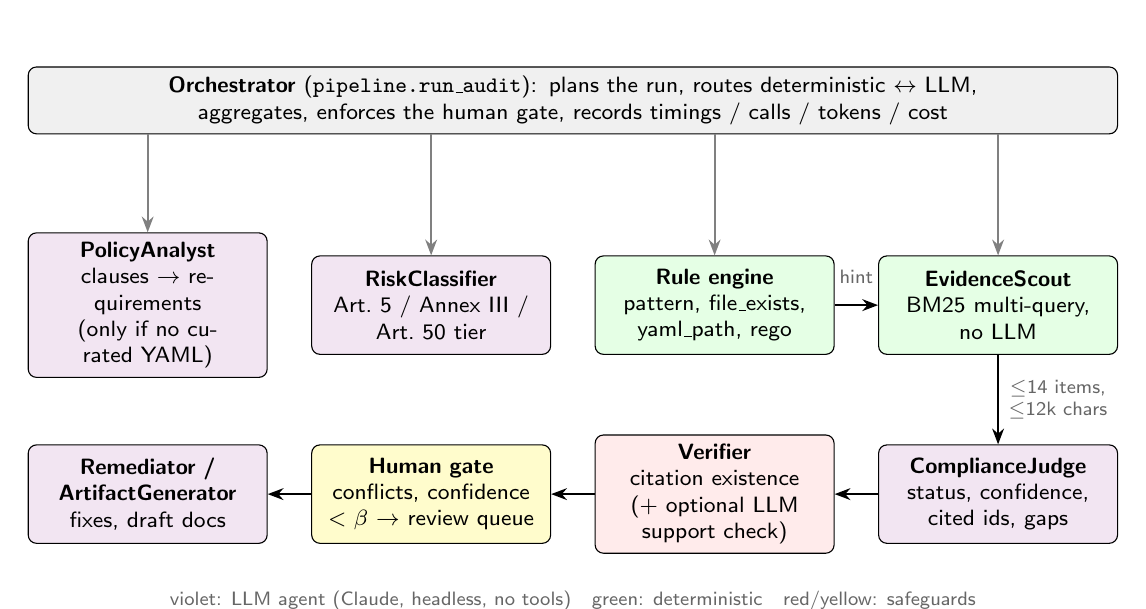
\begin{tikzpicture}[font=\sffamily\footnotesize,
  ag/.style={draw, rounded corners=3pt, fill=#1, align=center, text width=2.8cm, minimum height=1.25cm},
  ag/.default=violet!10,
  det/.style={draw, rounded corners=3pt, fill=green!10, align=center, text width=2.8cm, minimum height=1.25cm},
  arr/.style={-{Stealth[length=2mm]}, thick}, lab/.style={font=\sffamily\scriptsize, text=black!60, align=center}]
  \node[ag=gray!12, text width=13.6cm, minimum height=0.8cm] (orch) at (5.4,2.6)
     {\textbf{Orchestrator} (\texttt{pipeline.run\_audit}): plans the run, routes deterministic $\leftrightarrow$ LLM,
      aggregates, enforces the human gate, records timings / calls / tokens / cost};
  \node[ag] (pa) at (0,0) {\textbf{PolicyAnalyst}\\clauses $\to$ requirements\\(only if no curated YAML)};
  \node[ag] (rc) at (3.6,0) {\textbf{RiskClassifier}\\Art.~5 / Annex III /\\Art.~50 tier};
  \node[det] (re) at (7.2,0) {\textbf{Rule engine}\\pattern, file\_exists,\\yaml\_path, rego};
  \node[det] (sc) at (10.8,0) {\textbf{EvidenceScout}\\BM25 multi-query,\\no LLM};
  \node[ag] (jd) at (10.8,-2.4) {\textbf{ComplianceJudge}\\status, confidence,\\cited ids, gaps};
  \node[ag=red!8] (vf) at (7.2,-2.4) {\textbf{Verifier}\\citation existence\\(+ optional LLM support check)};
  \node[ag=yellow!20] (hl) at (3.6,-2.4) {\textbf{Human gate}\\conflicts, confidence\\$<\beta$ $\to$ review queue};
  \node[ag] (rm) at (0,-2.4) {\textbf{Remediator /}\\\textbf{ArtifactGenerator}\\fixes, draft docs};
  \foreach \n in {pa,rc,re,sc} \draw[arr, black!50] (orch.south -| \n) -- (\n);
  \draw[arr] (re) -- node[lab, above=4pt]{hint} (sc);
  \draw[arr] (sc) -- node[lab, right]{$\le$14 items,\\$\le$12k chars} (jd);
  \draw[arr] (jd) -- (vf);
  \draw[arr] (vf) -- (hl);
  \draw[arr] (hl) -- (rm);
  \node[lab] at (5.4,-3.75) {violet: LLM agent (Claude, headless, no tools)\quad green: deterministic\quad red/yellow: safeguards};
\end{tikzpicture}}
\caption{Agents of the auditor. Every LLM agent is a single structured (JSON-schema) call without tool access; the
orchestrator is ordinary code, so the control flow is fixed and auditable.}
\label{fig:agents}
\end{figure}

\section{Policy ingestion and decomposition}
\label{section:policies}

Policies are stored as markdown with a YAML front matter (\texttt{id}, \texttt{version}, \texttt{source}); headings
``\texttt{\#\# Art.~12 | Record-keeping}'' and ``\texttt{\#\#\# 1}'' are parsed into clauses with stable, citable ids
(\texttt{eu-ai-act/Art.12}, \texttt{eu-ai-act/Art.12(1)}) and parent links. Requirements are \emph{curated} in YAML
(statement, clause ids, category, applicable risk tiers, severity, retrieval queries, judge guidance and deterministic
checks). When no curated file exists for a policy, the \textbf{PolicyAnalyst} agent decomposes the clauses in batches,
with the instruction to emit only atomic, repository-testable requirements, to use only the given clause ids and to skip
definitional or authority-facing clauses. Table~\ref{tab:corpus} summarises the bundled corpus. A \textbf{policy
evolution} module diffs two versions of a policy at clause level (added / removed / modified, with parent--child
propagation) and lists the requirements and existing reports impacted by the change.

\begin{table}[htbp]
\caption{Policy corpus and curated requirements.}
\label{tab:corpus}
\centering\small
\begin{tabular}{@{}lrrrrl@{}}
\toprule
\textbf{Policy} & \textbf{Clauses} & \textbf{Req.} & \textbf{with checks} & \textbf{checks} & \textbf{check types} \\
\midrule
EU AI Act (selected provisions) & 108 & 23 & 22 & 25 & 19 pattern, 6 file\_exists \\
GDPR (selected articles) & 32 & 11 & 10 & 12 & 9 pattern, 3 file\_exists \\
ACME RAI policy (fictional, v1) & 30 & 11 & 10 & 12 & 11 pattern, 1 file\_exists \\
\midrule
\textbf{Total} & 170 & 45 & 42 & 49 & \\
\bottomrule
\end{tabular}
\end{table}

\section{Evidence collection and retrieval}
\label{section:evidence}

The collector walks the repository (skipping binaries, vendored and build directories), classifies each file into one of
six evidence kinds (code, config, IaC, doc, model card, log) and splits it into overlapping windows of 40 lines (overlap
10; files of at most 50 lines are a single chunk). Each chunk receives a stable id (hash of path and line span) and the
set of \emph{signals} raised by 16 lightweight regex detectors (logging call, AI disclosure, human override, retention
configuration, PII field, model call, consent, encryption, access control, rate limit, data documentation,
bias/fairness, accuracy metrics, risk management, monitoring, anonymisation).

Retrieval uses BM25~\cite{robertson2009bm25} over path + snippet with a code-aware tokenizer (camelCase and snake\_case
are split, the joined form is kept), boosted by $1.5\times$ when a query term matches a chunk signal. The
\textbf{EvidenceScout} builds several queries per requirement (curated queries, keywords of title + statement, one
category-specific expansion), merges the hits with a reciprocal-rank bonus, \emph{pins} the evidence already cited by the
rule engine first, and caps the result at 14 items and 12\,000 characters (1\,500 per snippet). No embedding model is
needed and the scout makes no LLM call.

\section{Risk-tier classification}
\label{section:risk}

Applicability depends on the AI Act tier. A deterministic pre-classifier matches regex triggers for prohibited practices
(Art.~5: social scoring, manipulation, workplace emotion recognition, untargeted facial scraping, predictive policing,
real-time remote biometric identification), Annex~III high-risk areas (biometrics, critical infrastructure, education,
employment, credit scoring, \dots) and Art.~50 transparency cases (chatbots, generative content, deep fakes) mostly in
documentation. Negated mentions are ignored (``the system does not interact with people as a chatbot'') and matches
are weighted by where they occur: a self-description in the README or model card counts 2.0, other documents 1.0 and
code 0.5, capped at 1.0 for code alone. A tier needs a score of at least 2. The classifier returns the most severe tier
together with the triggering evidence. In LLM modes the \textbf{RiskClassifier}
agent receives this result as a hint plus retrieved descriptions of the intended purpose, and returns tier, triggers and
cited evidence. Requirements whose $A_r$ excludes the tier get \stat{na} deterministically (Eq.~\ref{eq:applic}); the
judge is not allowed to output \stat{na}.

\section{Deterministic rule engine}
\label{section:rules}

Each check returns \emph{pass}, \emph{fail} or \emph{unknown}: \texttt{pattern} (a regex must be present / absent in files
selected by glob or evidence kind), \texttt{file\_exists}, \texttt{yaml\_path} (a key exists or equals a value in
YAML/JSON) and \texttt{rego} (evaluated with OPA~\cite{opa} if installed, otherwise unknown). Results are aggregated per
requirement: all resolved checks pass $\Rightarrow$ \stat{c}; none pass $\Rightarrow$ \stat{nc}; mixed $\Rightarrow$
\stat{p}; no resolved check $\Rightarrow$ \stat{nr}. The engine cites the matching chunks and lists the failed
checks as gaps.

\paragraph{Comment awareness.} Pattern checks run on a copy of each file in which comments, docstrings and
TODO/FIXME/TBD lines are blanked out; line numbers are preserved. Python is handled with \texttt{tokenize}; C-like,
hash, HCL, SQL and markup comments are handled by a string-aware scanner. Commented-out code and TODOs are treated as
non-evidence. Explanatory prose comments count only as a weak claim. Switched-off flags such as
\texttt{override\_allowed = False} do not satisfy a ``present'' check.

\paragraph{Graded confidence.} Each check outcome carries a strength. It depends on the number of matching lines and
files, on the evidence kind (a technical requirement satisfied only by documentation is a \emph{claim}, 0.55) and on
the check type (regex miss 0.6, ``absent'' pass 0.6, file exists 0.7, \dots). The verdict's confidence is the mean
strength of its decisive checks, plus $0.05$ when at least two independent checks agree, capped at $0.95$. \stat{p} and
\stat{nr} keep defaults of $0.5$ and $0.2$. The baseline (v0) instead used fixed priors: $0.9$ for \stat{c} and $0.8$
for \stat{nc}.

\section{LLM judge}
\label{section:judge}

The \textbf{ComplianceJudge} receives one requirement (statement, guidance, the text of its source clauses), the scout's
evidence rendered with short aliases (\texttt{[E1]}, \texttt{[E2]}, \dots, which are far less error-prone than hash ids),
and, in hybrid mode, the rule-engine verdict explicitly labelled as a hint that ``can be wrong (regexes are shallow)''.
The system prompt fixes the contract:
\begin{itemize}[leftmargin=*]
  \item decide only from the excerpts and cite only the given ids;
  \item absence of evidence is not compliance;
  \item use \stat{nr} only for genuinely ambiguous evidence;
  \item report a calibrated confidence (below 0.6 when unsure);
  \item list concrete gaps and an actionable remediation.
\end{itemize}
It also states the labelling rubric:
\begin{itemize}[leftmargin=*]
  \item the statement is the test, so the judge must not demand more than it says;
  \item an excerpt truncated at a chunk boundary is not a gap;
  \item claims and TODOs are not evidence;
  \item \stat{c}, \stat{p} and \stat{nc} have explicit meanings, and a missing artefact is \stat{nc}.
\end{itemize} The answer must follow a JSON schema
(\texttt{status, confidence, rationale, evidence\_ids, gaps, remediation}); aliases are mapped back to evidence ids, and
unknown ids are kept verbatim so that the Verifier can remove them.

\section{Hybrid orchestration}
\label{section:hybrid}

Algorithm~\ref{alg:hybrid} gives the orchestration. Two thresholds control the trade-off between cost and quality.
\begin{itemize}[leftmargin=*]
  \item The \emph{routing threshold} $\tau=0.675$ applies to the graded rule confidence. It was chosen by
        leave-one-app-out cross-validation (Section~\ref{section:results}) and sends about 60\% of the applicable items
        to the judge. Every \stat{p} or \stat{nr} rule verdict, and every requirement that has judge guidance but no
        checks, is always routed.
  \item The \emph{human-review threshold} is $\beta=0.6$.
\end{itemize}
The \textsc{Combine} step arbitrates transparently. On a hard disagreement (\stat{c} vs.\ \stat{nc}), the side that is
at least $\delta=0.15$ more confident wins; its confidence is lowered by $0.1$ and both rationales are recorded.
Otherwise the item becomes \stat{nr} for a reviewer. When the rules and the judge agree, the confidence rises by
$0.05$.

\algsetup{indent=1.5em, linenosize=\footnotesize}
\begin{algorithm}[htbp]
\caption{Hybrid audit orchestration (\texttt{pipeline.run\_audit}, mode = hybrid)}
\label{alg:hybrid}
\begin{algorithmic}[1]
\REQUIRE repository $D$, policy ids, LLM backend $B$, thresholds $\tau=0.675$, $\beta=0.6$, margin $\delta=0.15$
\ENSURE audit report with verdicts $V$, scorecard, statistics
\STATE $\Req \leftarrow$ curated requirements, or \textsc{PolicyAnalyst}$_B$(clauses) if none
\STATE $\Ev \leftarrow \varphi(D)$; build BM25 index over $\Ev$
\STATE $t \leftarrow$ \textsc{RiskClassifier}$_B$($\Ev$, hint = \textsc{HeuristicTier}($\Ev$))
\STATE $J \leftarrow \emptyset$ \COMMENT{requirements routed to the LLM judge}
\FORALL{$r \in \Req$}
  \IF{$t \notin A_r$}
    \STATE $V[r] \leftarrow (\stat{na}, \text{conf}(t), \emptyset)$; \textbf{continue}
  \ENDIF
  \STATE $d_r \leftarrow$ \textsc{Verify}(\textsc{RuleEngine}($r, D, \Ev$), ids$(\Ev)$, requireEvidence = false)
  \IF{$d_r.\text{status}\in\{\stat{p},\stat{nr}\}$ \OR $d_r.\text{conf} < \tau$ \OR ($K_r=\emptyset$ \AND $g_r \neq \varepsilon$)}
    \STATE $J \leftarrow J \cup \{r\}$
  \ELSE
    \STATE $V[r] \leftarrow d_r$ \COMMENT{confident rule verdict, no LLM call}
  \ENDIF
\ENDFOR
\FORALL{$r \in J$ \textbf{in parallel} (bounded by the backend concurrency)}
  \STATE $\Ev_r \leftarrow$ \textsc{EvidenceScout}($r$, pinned $=d_r$.ids) \COMMENT{BM25, $\le 14$ items}
  \STATE $\ell_r \leftarrow$ \textsc{ComplianceJudge}$_B$($r$, $\Ev_r$, hint $=d_r$)
  \STATE $\ell_r \leftarrow$ \textsc{Verifier}($r$, $\ell_r$, $\Ev_r \cup d_r$.ids) \COMMENT{Algorithm~\ref{alg:verifier}}
  \IF{$\{d_r.\text{status}, \ell_r.\text{status}\} = \{\stat{c},\stat{nc}\}$}
    \IF{$|\ell_r.\text{conf} - d_r.\text{conf}| \ge \delta$}
      \STATE $v \leftarrow$ more confident side, conf $- 0.1$, keep both rationales
    \ELSE
      \STATE $v \leftarrow (\stat{nr}, \min(0.5, d_r.\text{conf}, \ell_r.\text{conf}))$, keep both rationales
    \ENDIF
  \ELSIF{$d_r.\text{status} = \ell_r.\text{status}$}
    \STATE $v \leftarrow \ell_r$ with conf $\leftarrow \min(1, \max(d_r.\text{conf}, \ell_r.\text{conf}) + 0.05)$
  \ELSE
    \STATE $v \leftarrow \ell_r$ \COMMENT{e.g.\ rule \stat{p}, judge \stat{c}}
  \ENDIF
  \STATE $v \leftarrow$ \textsc{Verify}($v$, $\Ev_r \cup d_r$.ids)
  \IF{$v.\text{status}\notin\{\stat{nr},\stat{na}\}$ \AND $v.\text{conf} < \beta$}
    \STATE $v.\text{status} \leftarrow \stat{nr}$ \COMMENT{human-in-the-loop gate}
  \ENDIF
  \STATE $V[r] \leftarrow v$
\ENDFOR
\STATE scorecard $\leftarrow$ \textsc{Score}($\Req, V$); record timings, calls, tokens, cost, cache hits
\RETURN report($t$, $V$, cited evidence, scorecard, statistics)
\end{algorithmic}
\end{algorithm}

\section{Verifier: anti-hallucination contract}
\label{section:verifier}

The Verifier (Algorithm~\ref{alg:verifier}) enforces Eqs.~(\ref{eq:ground})--(\ref{eq:support}). Its deterministic pass
runs on \emph{every} verdict, including rule-engine ones: citations that do not belong to the evidence actually shown to
the evaluator are removed and the confidence is multiplied by $0.8$; a positive verdict (\stat{c} or \stat{p}) without
any remaining valid citation is downgraded to \stat{nr} with confidence at most $0.4$ (``no hallucinated compliance'').
An optional LLM pass, in the spirit of attribution checking~\cite{rashkin2023ais,min2023factscore}, shows a second,
sceptical model only the cited excerpts and asks whether they support the claim; unsupported claims become \stat{nr}
while the citations stay visible to the reviewer.

\begin{algorithm}[htbp]
\caption{Verifier (\texttt{agents/verifier.py})}
\label{alg:verifier}
\begin{algorithmic}[1]
\REQUIRE requirement $r$, verdict $v=(y,\pi,\hat E)$, evidence set provided to the evaluator $\Ev_r$, flag \textit{useLLM}
\ENSURE verified verdict
\STATE \textsc{Check}:
\STATE \quad $\hat E_{\text{bad}} \leftarrow \hat E \setminus \Ev_r$; \quad $\hat E \leftarrow \hat E \cap \Ev_r$
\IF{$\hat E_{\text{bad}} \neq \emptyset$}
  \STATE $\pi \leftarrow 0.8\,\pi$; append ``removed $|\hat E_{\text{bad}}|$ citation(s)'' to the rationale
\ENDIF
\IF{\textit{requireEvidence} \AND $y \in \{\stat{c}, \stat{p}\}$ \AND $\hat E = \emptyset$}
  \STATE $y \leftarrow \stat{nr}$; $\pi \leftarrow \min(\pi, 0.4)$ \COMMENT{no compliance without evidence}
\ENDIF
\STATE mark $v$ as verified
\IF{\textit{useLLM} \AND $y \in \{\stat{c}, \stat{p}\}$}
  \STATE $(s, U) \leftarrow$ LLM(``do excerpts $\hat E$ support status $y$ for statement $s_r$?'')
  \STATE $\hat E \leftarrow \hat E \setminus U$
  \IF{$s = \text{false}$ \OR $\hat E = \emptyset$}
    \STATE $y \leftarrow \stat{nr}$; $\pi \leftarrow \min(\pi, 0.5)$; keep original citations for the reviewer
  \ENDIF
\ENDIF
\RETURN $(y, \pi, \hat E)$
\end{algorithmic}
\end{algorithm}

\section{Human review, scoring and reporting}
\label{section:report}

Every verdict carries status, confidence, method (deterministic / llm / hybrid / human), a \emph{verified} flag,
rationale, gaps, remediation and the cited evidence with path and line span. Reviewers resolve \stat{nr} items (or
contest any other verdict) by submitting a decision with their name and a justification; the override is recorded in the
rationale and in the report history, the method becomes \texttt{human} and the scorecard is recomputed. Category scores
are $(\#\stat{c} + 0.5\,\#\stat{p}) / \#\text{applicable} \times 100$; the overall score uses the same credit weighted by
severity (critical 4, high 3, medium 2, low 1). Reports are rendered as JSON, Markdown and SARIF~\cite{sarif2020} (so
that gaps appear as code-scanning alerts on the cited lines), and an \texttt{explain} function prints the full
justification of a single verdict. The \textbf{ArtifactGenerator} drafts missing artefacts (technical documentation,
risk assessment, transparency notice, model card~\cite{mitchell2019modelcards}) from the findings, with explicit
\texttt{[TODO]} placeholders instead of invented facts.

\section{LLM backend, caching and CI}
\label{section:backend}

The LLM is Claude, called through the \textbf{Claude Code CLI in headless mode}~\cite{claudecode}
(\texttt{claude -p --output-format json --json-schema ...}) with the developer's subscription, so no API key is stored.
Each call runs with tools, MCP servers, slash commands, settings and session persistence disabled, in an empty temporary
working directory: the model can read only the prompt. Responses are parsed (with a fallback that extracts the first
balanced JSON object), validated against the schema and retried up to twice with the validation errors appended. A
content-addressed \textbf{disk cache} (SHA-256 of model, system prompt, prompt and schema) makes re-audits of unchanged
code free and deterministic; the backend records calls, cache hits, failures, input/output tokens, the equivalent USD
cost reported by the CLI and latency. A semaphore bounds the concurrency (default 4). A \texttt{FakeBackend} makes the
whole pipeline testable offline. In CI, \texttt{ccauditor ci} audits the current tree, compares it with a baseline report
(per-requirement status rank $\stat{nc} < \stat{nr} < \stat{p} < \stat{c}$) and fails the build on regressions at or above
a chosen severity.

\section{Web dashboard}
\label{section:web}

The Next.js dashboard (over the REST API: \texttt{/policies}, \texttt{/audit}, \texttt{/reports/compare},
\texttt{/reports/render}, \texttt{/reports/review}, \texttt{/policies/diff}) lets a user browse policies and clauses, launch
an audit (mode, policies, model), and inspect a report in four tabs: \emph{overview} (score gauge, per-category charts, risk
tier and triggers), \emph{requirements} (filterable table; a side sheet shows the statement, source clauses, rationale,
cited code snippets, gaps and remediation), \emph{review} (the human-in-the-loop queue with a decision form) and
\emph{traceability} (clause $\to$ requirement $\to$ evidence links). Figure~\ref{fig:dashboard} shows the report of
\texttt{hireright-screening} in hybrid mode.

\begin{figure}[htbp]
\centering
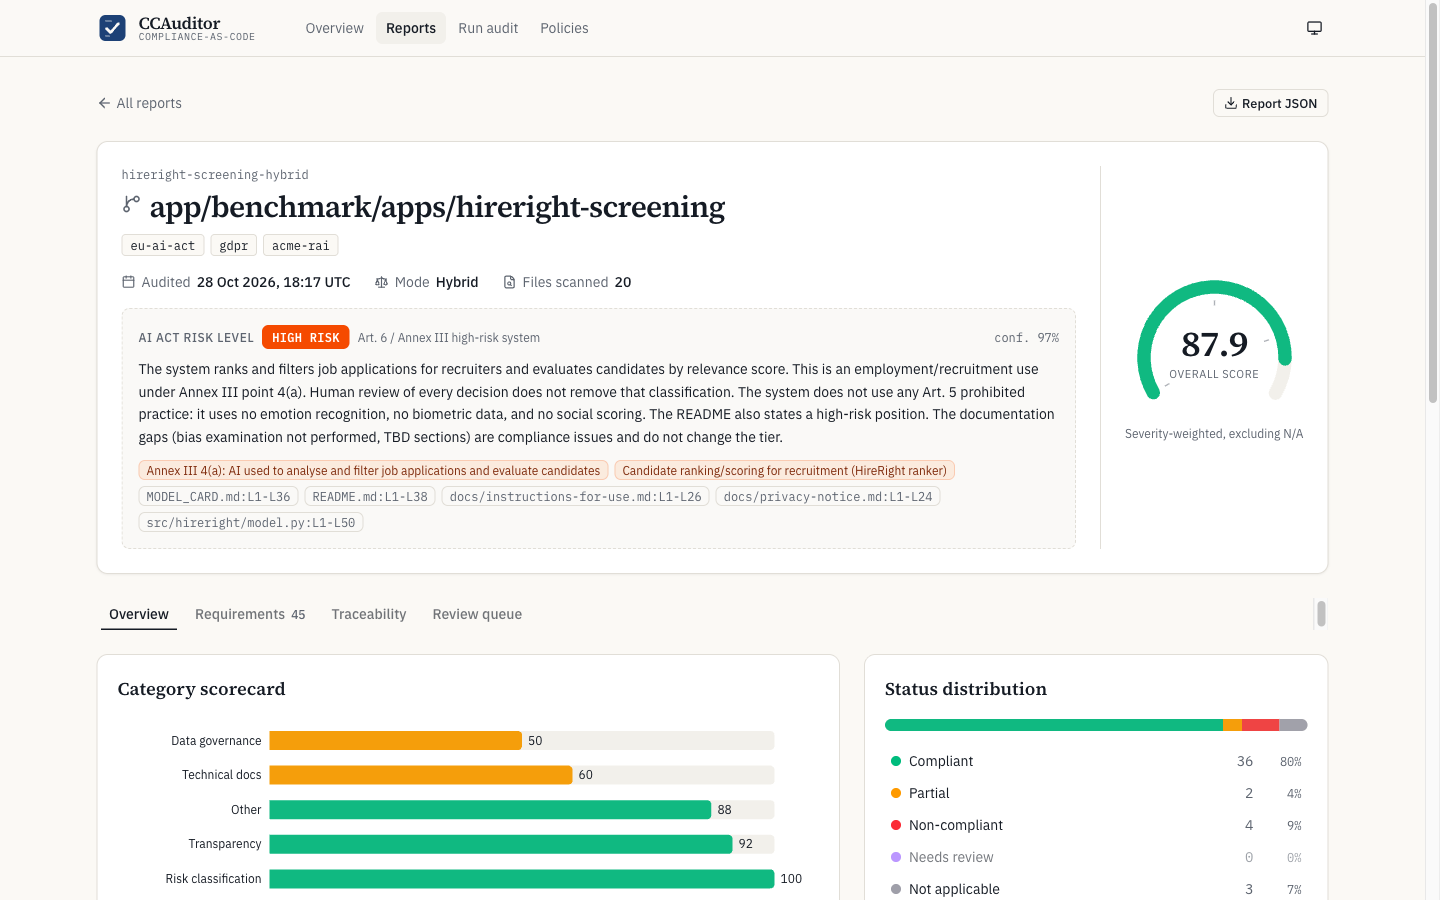
\includegraphics[width=0.6\linewidth]{figures/dashboard_overview.png}\hfill
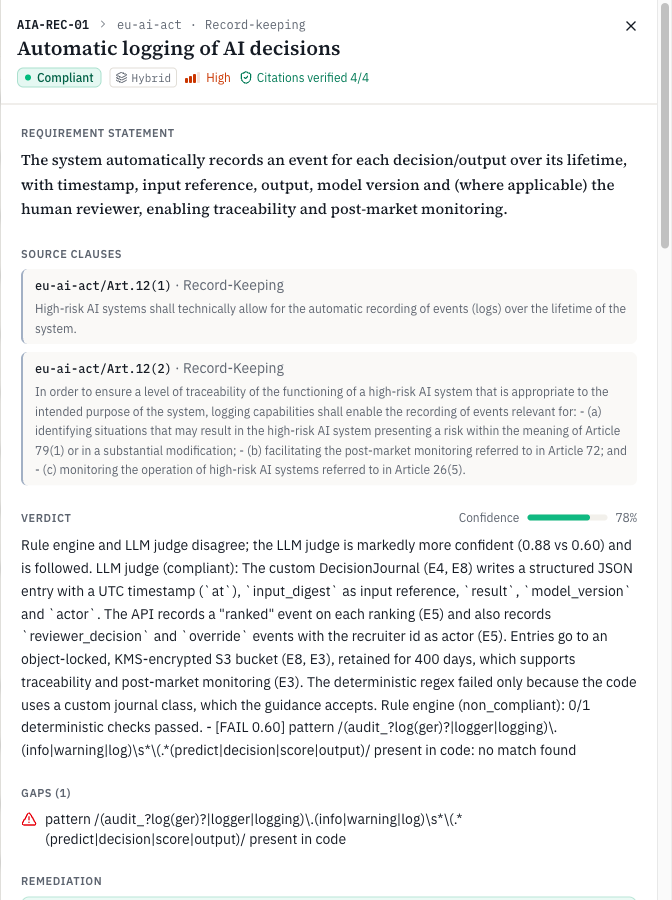
\includegraphics[width=0.38\linewidth]{figures/dashboard_requirement.png}
\caption{Web dashboard, \texttt{hireright-screening} audited in hybrid mode. Left: the overview, with the risk tier, its
triggers and cited files, the severity-weighted score and the category scorecard. Right: the requirement drawer for
\texttt{AIA-REC-01}, showing the statement, the source clauses, the verdict with its confidence and the arbitration
rationale (rule engine vs.\ LLM judge), verified citations and gaps. Further down the drawer are the cited code and
the human-review form.}
\label{fig:dashboard}
\end{figure}

\section{Worked example}
\label{section:example}

Consider requirement \texttt{AIA-REC-01} on \texttt{hireright-screening}, a high-risk CV-ranking service (Annex~III
4(a)). The requirement derives from Art.~12(1)--(2): every decision must be logged automatically with a timestamp, an
input reference, the output and the model version. The ground truth is \stat{c}, because every ranking is recorded by a
custom \texttt{DecisionJournal.record(...)} on S3 Object Lock, and no \texttt{logger} call is used.
\begin{enumerate}[leftmargin=*]
  \item The tier is \emph{high}, triggered by the recruitment description in the README and the model card, so the
        requirement applies.
  \item The rule check is a regex for a \texttt{logger} or \texttt{audit\_log} call in code that mentions a prediction,
        decision, score or output. It does not match, so the rule engine says \stat{nc}.
  \item \textbf{v0:} the fixed prior gave this verdict confidence $0.8 \ge 0.75$, so hybrid mode kept the confident but
        wrong \stat{nc} without asking the LLM. The deterministic and hybrid modes were both wrong. LLM-only mode was
        right (\stat{c}, 0.82, 5 citations).
  \item \textbf{v1:} a regex miss is graded at $0.6 < \tau$, so the item is routed. The scout's queries ``journal
        record decision'' and ``audit log decision'' retrieve \texttt{journal.py}, the call sites in \texttt{api.py}
        and the retention configuration. The judge answers \stat{c} with confidence 0.88 and cites 4 excerpts. The
        judge is $0.28 \ge \delta$ more confident than the rules, so it wins the arbitration. The final verdict is
        \stat{c} with confidence 0.78, and both rationales stay visible (Figure~\ref{fig:dashboard}, right).
\end{enumerate}
The example shows the central trade-off quantified in Chapter~\ref{chapter:experiments}. Confident rules save LLM calls
but propagate their false negatives. Graded confidence makes a ``regex miss'' weak enough to be checked, while strong
rule evidence still saves the call.

\chapter{Experiments}
\label{chapter:experiments}

\section{Research questions and hypotheses}
\label{section:hypotheses}

\begin{description}[leftmargin=1.2cm, labelwidth=1cm]
  \item[RQ1] \emph{Quality.} Does the hybrid mode reach at least the accuracy and macro-F1 of the LLM-only mode, and
        exceed the deterministic mode, on applicable requirements?
  \item[RQ2] \emph{Safety.} Which mode minimises the false-compliance rate, and how much human workload (needs-review
        rate) does that cost?
  \item[RQ3] \emph{Cost.} How many LLM calls, tokens, dollars and seconds does each mode need per audit, and how much does
        the cache save on a re-audit?
  \item[RQ4] \emph{Safeguards.} What do the Verifier, the LLM support check and the model size contribute (ablations)?
\end{description}
\noindent The \emph{independent variables} are the mode, the model, and the safeguard switches; the \emph{dependent
variables} are the metrics of Section~\ref{section:formal}.

\section{Data: a hand-labelled benchmark}
\label{section:data}

There is no public dataset of application repositories labelled against the AI Act, so we built one
(\texttt{app/benchmark}). Five small but realistic repositories cover the four risk tiers and different stacks
(Table~\ref{tab:apps}); each contains code, configuration, infrastructure-as-code, documentation, model cards and sample
logs as real teams would write them. Every one of the 45 curated requirements was labelled for every app (225 labels,
165 applicable), with a justification and file references. Labels were written \emph{before} running the rule engine, by
reading the repository against the requirement statement; claims without backing (README marketing, TODOs, commented code)
are not evidence; \stat{na} is used only when the requirement's risk tiers exclude the app's tier, so it is never a
judgement call. Table~\ref{tab:labels} gives the label distribution.

\begin{table}[htbp]
\caption{Benchmark applications.}
\label{tab:apps}
\centering\small
\begin{tabularx}{\linewidth}{@{}lllX@{}}
\toprule
\textbf{App} & \textbf{Domain} & \textbf{AI Act tier} & \textbf{Compliance profile} \\
\midrule
\texttt{hireright-screening} & CV ranking & high (Annex III 4(a)) & mostly compliant; logging via a custom journal, kill switch with an unusual name; gaps: bias evaluation, ROPA, DPIA \\
\texttt{quickhire-ranker} & CV ranking MVP & high (Annex III 4(a)) & mostly non-compliant: auto-rejection, protected attributes as features, no auth; decoys (commented logger, ``fully GDPR compliant'' README) \\
\texttt{supportbot-genai} & support chatbot & limited (Art.~50) & disclosure banner, erasure endpoint; gaps: unlabelled AI replies (TODO only), 2-year transcript retention \\
\texttt{credit-lens} & credit scoring & high (Annex III 5(b)) & strong governance; gaps: 30-day log retention, automatic declines up to EUR 25\,000, no instructions for use \\
\texttt{spamshield} & spam filter & minimal & most AI Act duties N/A; GDPR largely compliant; gaps: incident procedure, on-request erasure \\
\bottomrule
\end{tabularx}
\end{table}

\begin{table}[htbp]
\caption{Ground-truth label distribution (45 requirements $\times$ 5 apps).}
\label{tab:labels}
\centering\small
\begin{tabular}{@{}llrrrrr@{}}
\toprule
\textbf{App} & \textbf{Tier} & \stat{c} & \stat{p} & \stat{nc} & \stat{na} & \textbf{total} \\
\midrule
credit-lens & high & 32 & 7 & 3 & 3 & 45 \\
hireright-screening & high & 37 & 1 & 4 & 3 & 45 \\
quickhire-ranker & high & 1 & 2 & 39 & 3 & 45 \\
spamshield & minimal & 15 & 2 & 1 & 27 & 45 \\
supportbot-genai & limited & 15 & 2 & 4 & 24 & 45 \\
\midrule
\textbf{all} & & \textbf{100} & \textbf{14} & \textbf{51} & \textbf{60} & \textbf{225} \\
\bottomrule
\end{tabular}
\end{table}

The benchmark is deliberately adversarial for rules: \emph{indirect evidence} (regex false negatives, e.g.\ a
\texttt{DecisionJournal} instead of \texttt{logger}, ``pseudonymous'' instead of ``pseudonymise''), \emph{decoys} (regex
false positives, e.g.\ \texttt{\# logger.info(...)}, \texttt{override\_allowed = False}, a TODO to label AI replies) and
three requirements without any check. It is also adversarial for LLMs: plausible but unbacked claims in READMEs and
disproportionate-but-present controls (retention defined but too long) that require reading thresholds.

\subsection{Exploratory data analysis}
\label{section:eda}

Figures~\ref{fig:eda-corpus}--\ref{fig:eda-signals} describe the inputs. The AI Act dominates the corpus, with long and
structurally varied clauses (Annex~III, Art.~9, Art.~13). Most requirements have exactly one deterministic check, and three
have none (Figure~\ref{fig:eda-corpus}). The applications differ in the mix of evidence kinds: \texttt{hireright} and
\texttt{credit-lens} are documentation-heavy, \texttt{quickhire} is mostly code (Figure~\ref{fig:eda-bench}). The labels
are imbalanced per application by design (Figure~\ref{fig:eda-labels}). The signal heat map
(Figure~\ref{fig:eda-signals}) shows why a signal alone is weak evidence: for example, 50\% of \texttt{quickhire} chunks
carry a PII signal, yet that application has no data protection.

\begin{figure}[htbp]
\centering
\maybefig[0.49\linewidth]{eda_clauses}{Clauses per article and clause length.}\hfill
\maybefig[0.49\linewidth]{eda_requirements}{Requirements per category, severity, checks per requirement.}
\caption{Policy corpus: clauses per article and clause length (left); requirements per category, severity and number of
deterministic checks (right).}
\label{fig:eda-corpus}
\end{figure}

\begin{figure}[htbp]
\centering
\maybefig[0.8\linewidth]{eda_benchmark_files}{Files and evidence chunks per kind and app.}
\caption{Benchmark repositories: files and evidence chunks per evidence kind.}
\label{fig:eda-bench}
\end{figure}

\begin{figure}[htbp]
\centering
\maybefig[0.8\linewidth]{eda_labels}{Labels per app and applicable labels per category.}
\caption{Ground-truth labels per application (left) and applicable labels per category (right).}
\label{fig:eda-labels}
\end{figure}

\begin{figure}[htbp]
\centering
\maybefig[0.6\linewidth]{eda_signals}{Share of evidence chunks carrying each signal, per app.}
\caption{Share of evidence chunks carrying each collector signal, per application.}
\label{fig:eda-signals}
\end{figure}

\section{Protocol}
\label{section:protocol}

\begin{itemize}[leftmargin=*]
  \item \textbf{Configurations.} \emph{deterministic}; \emph{hybrid} and \emph{llm} with Claude Sonnet (default) and
        Claude Haiku (smaller, cheaper); all three policies at once on each app (45 requirements per audit).
  \item \textbf{Runs.} \texttt{app/benchmark/evaluate.py} audits the five apps in parallel processes (3 concurrent LLM
        calls per audit), stores every full report, the per-item predictions and a $5\times5$ confusion matrix per
        configuration. Temperature cannot be set through the CLI; variance is estimated by repeating cold (uncached)
        runs. \resultsTODO{number of repetitions and seeds.}
  \item \textbf{Ablations.} (a) Verifier disabled (\texttt{--no-verifier}); (b) LLM claim-support check enabled
        (\texttt{--verify-llm}); (c) model size (Sonnet vs.\ Haiku); (d) routing threshold $\tau$ / routing of confident
        \stat{nc} rule verdicts; (e) cache: cold run vs.\ warm re-audit of unchanged code.
  \item \textbf{Statistics.} 95\% bootstrap confidence intervals over items (1\,000 resamples) for accuracy, macro-F1 and
        FCR, and McNemar's exact test on paired per-item correctness between modes.
  \item \textbf{Hardware.} \todo{CPU / RAM / OS of the machine}; LLM inference runs on Anthropic's servers via the
        Claude Code CLI \todo{CLI version}, so local memory is dominated by the Python process.
\end{itemize}

\section{Results}
\label{section:results}

\IfFileExists{results_tables.tex}{% Main results. Source: app/benchmark/results/SUMMARY.md (v0_baseline.json, v1_improved.json) and
% app/benchmark/results/stats_tests.json (app/benchmark/stats_tests.py).
Table~\ref{tab:main-results} gives all configurations on the 165 applicable labels; Table~\ref{tab:stats} adds 95\%
bootstrap confidence intervals and paired McNemar tests.

\begin{table}[htbp]
\caption{Results on the 165 applicable labels (percentages). Cost is the equivalent USD reported by the CLI for the
five audits (cached calls counted at their original cost); s/app is the wall-clock per app audit of a cold run.
v0 = baseline, v1 = improved system (Section~\ref{section:v1}). Best v1 value per column in bold.}
\label{tab:main-results}
\centering\scriptsize
\setlength{\tabcolsep}{3.2pt}
\resizebox{\linewidth}{!}{%
\begin{tabular}{@{}llrrrrrrrrrr@{}}
\toprule
& \textbf{Config} & \textbf{Acc} & \textbf{M-F1} & \textbf{Gap P} & \textbf{Gap R} & \textbf{FCR}$\downarrow$ & \textbf{NR} & \textbf{Acc@def} & \textbf{Calls} & \textbf{Cost \$} & \textbf{s/app} \\
\midrule
\multirow{3}{*}{v0} & deterministic & 79.4 & 72.3 & 78.1 & 87.7 & 12.3 & 5.5 & 84.0 & 0 & 0.00 & 0.2 \\
& hybrid (Sonnet) & 86.1 & 77.1 & 83.8 & 87.7 & 12.3 & 0.0 & 86.1 & 23 & 0.67 & 25 \\
& llm (Sonnet) & 71.5 & 67.6 & 60.8 & \textbf{100.0} & \textbf{0.0} & 0.6 & 72.0 & 170 & 4.81 & 94 \\
\midrule
\multirow{5}{*}{v1} & deterministic & 82.4 & 74.9 & 80.3 & 93.8 & 6.2 & 5.5 & 87.2 & 0 & \textbf{0.00} & \textbf{0.2} \\
& \textbf{hybrid (Sonnet)}, $\tau=0.675$ & \textbf{94.5} & \textbf{86.6} & \textbf{96.9} & 96.9 & 3.1 & 0.6 & \textbf{95.1} & 103 & 2.77 & 50 \\
& llm (Sonnet) & 90.9 & 83.1 & 85.5 & \textbf{100.0} & \textbf{0.0} & 0.6 & 91.5 & 170 & 4.68 & 91 \\
& hybrid (Haiku) & 83.6 & 75.4 & 76.8 & 96.9 & 3.1 & 5.5 & 88.5 & 103 & 0.19 & 75 \\
& llm (Haiku) & 71.5 & 66.7 & 61.9 & \textbf{100.0} & \textbf{0.0} & 7.3 & 77.1 & 170 & 0.32 & 116 \\
\midrule
\multirow{3}{*}{\shortstack[l]{v1\\ablation}} & hybrid (Sonnet), route all ($\tau>1$) & 90.9 & 82.1 & 87.7 & 98.5 & 1.5 & 0.6 & 91.5 & 170 & 4.82 & 90 \\
& hybrid (Sonnet), no Verifier & 94.5 & 86.6 & 96.9 & 96.9 & 3.1 & 0.6 & 95.1 & 103 & 2.77 & 50 \\
& hybrid (Sonnet) + LLM claim verifier & 88.5 & 83.1 & 85.1 & 96.9 & 3.1 & 6.7 & 94.8 & 156 & 3.89 & 89 \\
\bottomrule
\end{tabular}}
\end{table}

\noindent In every configuration the citation validity was 100\% (no cited id outside the evidence index) and in every v1
configuration that uses the LLM, every \stat{c} verdict cites at least one evidence item. Risk-tier
accuracy is 100\% for all v1 configurations (v0 deterministic: 80\%, \texttt{spamshield} classified as limited).

\begin{table}[htbp]
\caption{Statistical validation: 95\% percentile bootstrap CIs (10\,000 resamples of the 165 items) and exact
two-sided McNemar tests on paired per-item correctness ($b$: only A correct, $c$: only B correct).}
\label{tab:stats}
\centering\scriptsize
\begin{tabular}{@{}lccc@{}}
\toprule
\textbf{Configuration} & \textbf{Accuracy} & \textbf{Macro-F1} & \textbf{FCR} \\
\midrule
v0 deterministic & 79.4 [72.7, 85.5] & 72.3 [61.4, 81.6] & 12.3 [4.8, 20.9] \\
v0 llm (Sonnet) & 71.5 [64.8, 78.2] & 67.6 [61.0, 73.8] & 0.0 [0.0, 0.0] \\
v1 deterministic & 82.4 [76.4, 87.9] & 74.9 [64.2, 84.0] & 6.2 [1.4, 12.7] \\
v1 hybrid (Sonnet) & 94.5 [90.9, 97.6] & 86.6 [77.0, 94.1] & 3.1 [0.0, 7.9] \\
v1 llm (Sonnet) & 90.9 [86.7, 95.2] & 83.1 [74.6, 90.1] & 0.0 [0.0, 0.0] \\
v1 hybrid (Haiku) & 83.6 [77.6, 89.1] & 75.4 [66.8, 83.3] & 3.1 [0.0, 7.9] \\
\bottomrule
\end{tabular}
\vspace{0.6em}

\begin{tabular}{@{}llrrr@{}}
\toprule
\textbf{A} & \textbf{B} & $b$ & $c$ & \textbf{$p$-value} \\
\midrule
v1 hybrid (Sonnet) & v1 deterministic & 22 & 2 & $3.6\times10^{-5}$ \\
v1 hybrid (Sonnet) & v1 llm (Sonnet) & 11 & 5 & 0.21 \\
v1 hybrid (Sonnet) & v1 hybrid, route all & 7 & 1 & 0.070 \\
v1 hybrid (Sonnet) & v1 hybrid (Haiku) & 20 & 2 & $1.2\times10^{-4}$ \\
v1 hybrid (Sonnet) & v1 hybrid + LLM claim verifier & 10 & 0 & 0.0020 \\
v1 llm (Sonnet) & v0 llm (Sonnet) & 34 & 2 & $1.9\times10^{-8}$ \\
v1 hybrid (Sonnet) & v0 hybrid (Sonnet) & 16 & 2 & 0.0013 \\
v1 deterministic & v0 deterministic & 5 & 0 & 0.063 \\
\bottomrule
\end{tabular}
\end{table}
}{%
Table~\ref{tab:main-results} is filled from \texttt{app/benchmark/results/SUMMARY.md}.

\begin{table}[htbp]
\caption{Main results on the 165 applicable labels (percentages; cost and latency per app audit).}
\label{tab:main-results}
\centering\scriptsize
\setlength{\tabcolsep}{3.5pt}
\begin{tabular}{@{}lrrrrrrrrrr@{}}
\toprule
\textbf{Config} & \textbf{Acc} & \textbf{M-F1} & \textbf{Gap P} & \textbf{Gap R} & \textbf{FCR}$\downarrow$ & \textbf{NR} & \textbf{Acc@def} & \textbf{Cit.\ valid} & \textbf{LLM calls} & \textbf{Cost \$ / s} \\
\midrule
deterministic        & \res{} & \res{} & \res{} & \res{} & \res{} & \res{} & \res{} & \res{} & 0 & 0 / \res{} \\
hybrid (Sonnet)      & \res{} & \res{} & \res{} & \res{} & \res{} & \res{} & \res{} & \res{} & \res{} & \res{} \\
llm (Sonnet)         & \res{} & \res{} & \res{} & \res{} & \res{} & \res{} & \res{} & \res{} & \res{} & \res{} \\
hybrid (Haiku)       & \res{} & \res{} & \res{} & \res{} & \res{} & \res{} & \res{} & \res{} & \res{} & \res{} \\
\midrule
hybrid, no Verifier  & \res{} & \res{} & \res{} & \res{} & \res{} & \res{} & \res{} & \res{} & \res{} & \res{} \\
hybrid, LLM verifier & \res{} & \res{} & \res{} & \res{} & \res{} & \res{} & \res{} & \res{} & \res{} & \res{} \\
\bottomrule
\end{tabular}
\end{table}

\resultsTODO{fill Table~\ref{tab:main-results} (or provide \texttt{docs/report/results\_tables.tex}, which replaces this
block automatically), add bootstrap CIs and McNemar p-values.}
}

\begin{figure}[htbp]
\centering
\maybefig{mode_comparison}{Bar chart: accuracy, macro-F1, gap F1, FCR, needs-review per configuration.}
\caption{Quality metrics per configuration.}
\label{fig:mode-comparison}
\end{figure}

\begin{figure}[htbp]
\centering
\maybefig[0.48\linewidth]{confusion_hybrid}{Confusion matrix (truth $\times$ prediction) of the hybrid mode.}\hfill
\maybefig[0.48\linewidth]{confusion_llm}{Confusion matrix of the LLM-only mode.}
\caption{Confusion matrices (rows: ground truth, columns: prediction) for hybrid (left) and LLM-only (right).}
\label{fig:confusion}
\end{figure}

\begin{figure}[htbp]
\centering
\maybefig[0.7\linewidth]{cost_quality}{Scatter: cost (USD) or LLM calls per audit vs.\ accuracy / FCR, one point per configuration.}
\caption{Cost--quality trade-off of the configurations.}
\label{fig:cost-quality}
\end{figure}

\begin{figure}[htbp]
\centering
\maybefig{per_category}{Heat map or grouped bars: accuracy per requirement category and mode.}
\caption{Accuracy per requirement category.}
\label{fig:per-category}
\end{figure}

\section{Complexity and sustainability}
\label{section:complexity}

\paragraph{Time and memory.} The deterministic mode is CPU-only and runs in well under a second per application; memory
is bounded by the evidence index (a few thousand chunks for our apps). In LLM modes wall-clock time is dominated by the
judge calls and scales with the number of routed requirements divided by the concurrency.
\resultsTODO{per-stage timings (requirements, evidence, risk, deterministic, LLM judge, report) and peak RSS.}

\paragraph{Cost and energy.} Cost is measured as the equivalent USD reported by the CLI per call
(\texttt{total\_cost\_usd}; the subscription itself is a flat fee) together with input/output tokens. We cannot meter the
energy of a hosted model directly, so tokens and the number of calls are used as proxies: inference energy grows with
generated and processed tokens~\cite{luccioni2024power,strubell2019energy}. Three design choices reduce them: (1)
\emph{routing} -- the LLM sees only the requirements the rules cannot settle; (2) \emph{bounded prompts} -- at most 14
evidence items and 12\,000 characters per judgement, one requirement per call, no tool use; (3) a \emph{content-addressed
cache}, so a re-audit of an unchanged repository (the common CI case) costs no new calls.
\resultsTODO{cold vs.\ warm cost and calls per audit; tokens per configuration.}

\section{Explainability}
\label{section:explainability}

Every verdict is explainable by construction: it carries the rule-check trace (which check passed or failed and where),
the judge's rationale that refers to evidence aliases, the cited \texttt{file:line} snippets, the gaps and the
remediation; conflicts keep both the rule and the LLM rationale. \texttt{ccauditor explain} and the dashboard side sheet
render this justification for a single requirement, and SARIF places the finding on the cited lines in code review.

\section{Discussion}
\label{section:discussion}

\resultsTODO{answer RQ1--RQ4 with the numbers: is the hybrid hypothesis supported; where does each mode fail (per
category, per app); effect of the Verifier and of model size; statistical significance; cost per correct verdict.}

Independently of the final numbers, the design implies the following expected failure modes, which the analysis should
confirm or refute: (i) the rule engine is precise on decoy-free, syntactic requirements but propagates confident false
negatives on indirect evidence (Section~\ref{section:example}); (ii) the LLM-only mode recovers indirect evidence but
tends to be stricter, flagging more items as gaps (higher gap recall, lower gap precision) and costing an order of
magnitude more calls; (iii) the hybrid mode inherits the rule engine's confident errors because they are never routed,
which bounds its accuracy from above and is the main target for threshold tuning; (iv) data-governance and
human-oversight requirements are the hardest for rules, because their evidence is mostly prose.

\paragraph{Threats to validity.} The benchmark is small (5 apps, 225 labels), synthetic and labelled by the authors who
also wrote the rules, which risks optimistic results for the deterministic mode on the patterns we anticipated; we
mitigated this by labelling before running the rules and by planting traps against our own rules. Policies are selected
provisions, requirements are curated, and the AI Act will be complemented by harmonised standards that may change what
counts as sufficient evidence.

\chapter{Governance aspects}
\label{chapter:governance}

An AI system that audits AI systems must itself be governed. We analyse the auditor along the course's governance
dimensions; Table~\ref{tab:agency} summarises its agency.

\section{Ethics}
\label{section:ethics}

The main ethical risk is \emph{false assurance}: a report that says ``compliant'' where the law is not met can harm the
people affected by the audited system (rejected candidates, declined borrowers) and shift blame to a tool. We therefore
(i) treat a false compliance as the worst error in both the metrics and the design (no positive verdict without a
verified citation; disagreement $\Rightarrow$ human); (ii) state in every report that it is decision support for an
internal audit~\cite{raji2020closing}, not a conformity assessment or legal advice; (iii) never let generated artefacts
invent facts (explicit \texttt{[TODO]} placeholders). \emph{Privacy:} the auditor reads source repositories that may
contain secrets or personal data in sample logs; only bounded excerpts are sent to the LLM, through the user's own Claude
account, with no tool access and no session persistence, and the local cache can be disabled or wiped. A deployment on
confidential code should add secret/PII redaction before prompting, which is listed as future work. \emph{Dual use:} the
same tool could be used to produce a ``clean'' report by tuning rules to pass; the full rule trace and the report history
make such manipulation visible.

\section{Fairness}
\label{section:fairness}

Fairness concerns the auditor in two ways. First, \emph{fairness of the audited systems}: the requirements include data
governance and bias examination (AI Act Art.~10), and the benchmark contains a system that uses age, gender and nationality
as features; the auditor can check that bias evaluation is \emph{documented and performed}, but it does not measure bias
itself (it has no access to data or predictions), and it should not be read as a fairness certification~\cite{mehrabi2021survey}.
Second, \emph{fairness of the auditor across the audited}: the same requirement should receive the same verdict for
equivalent evidence regardless of programming language, documentation language or naming style. Rules are biased toward
the vocabulary they were written for (e.g.\ English identifiers, \texttt{logger}); the LLM is more robust to naming but
may favour verbose, well-documented repositories. We report per-category and per-application results to expose such
disparities; extending the benchmark to non-English documentation and more stacks is future work.

\section{Agency: what the system may decide and how far it may act}
\label{section:agency}

Following the levels-of-automation view of Parasuraman et al.~\cite{parasuraman2000levels}, the auditor automates
information acquisition and analysis fully, \emph{recommends} decisions, and \emph{executes} nothing.

\begin{table}[htbp]
\caption{Agency of the auditor: decisions it may take alone, with a human, or never.}
\label{tab:agency}
\centering\small
\begin{tabularx}{\linewidth}{@{}p{3.3cm}XX@{}}
\toprule
\textbf{Level} & \textbf{Decisions} & \textbf{Condition} \\
\midrule
Autonomous & collect evidence, classify risk tier, mark \stat{na}, emit \stat{c}/\stat{p}/\stat{nc} verdicts,
draft remediation and artefacts, fail a CI build on a regression & verdict verified, confidence $\ge \beta$, no rule/LLM
conflict; CI failure is reversible and threshold set by the team \\
Human-in-the-loop & any verdict with confidence $< \beta$, any rule vs.\ LLM conflict, any \stat{c} claim without valid
citation, contested verdicts & routed to the review queue as \stat{nr}; a named reviewer decides \\
Never & modify the audited repository, commit or merge, file anything with a regulator, declare legal conformity,
decide applicability by LLM alone & out of scope by design (no write tools; judge cannot output \stat{na}) \\
\bottomrule
\end{tabularx}
\end{table}

The system may therefore act \emph{only on its own outputs} (a report, a SARIF file, a CI exit code). The furthest it acts
before a person is involved is blocking a merge in CI, which is reversible, configurable (fail-on severity) and based on a
regression relative to a baseline that a human accepted.

\section{Architecture: components required by that permission}
\label{section:architecture-gov}

Each permission in Table~\ref{tab:agency} is backed by a concrete component:
\begin{itemize}[leftmargin=*]
  \item \textbf{Retrieval}: the evidence index and the BM25 EvidenceScout bound what the judge can see; every claim must be
        traceable to an indexed chunk with path and line span.
  \item \textbf{Tools}: none for the LLM. The Claude Code CLI runs with tools, MCP servers and settings disabled in an empty
        temporary directory; only the deterministic code reads files. This removes the risk of an agent modifying the repo.
  \item \textbf{Memory}: no conversational memory between calls (no session persistence); the only memory is the
        content-addressed response cache (reproducibility) and the stored reports with their review history
        (institutional memory, input to CI regression checks).
  \item \textbf{Orchestration}: a fixed, ordinary-code pipeline (Algorithm~\ref{alg:hybrid}) with explicit routing
        thresholds; agents cannot spawn agents or change the plan.
  \item \textbf{Checks}: JSON-schema validation with bounded retries, the Verifier (Algorithm~\ref{alg:verifier}), the
        conflict rule and the confidence gate, and the CI regression comparator.
\end{itemize}

\section{Accountability: who answers, what the record shows, how to contest}
\label{section:accountability}

Accountability for AI requires an identifiable answerable agent, a record and a forum~\cite{novelli2023accountability}.
\begin{itemize}[leftmargin=*]
  \item \textbf{Who answers.} The organisation deploying the audited system (the AI Act provider or deployer) remains
        responsible for compliance; within it, the named reviewer who resolves an item answers for that decision, and the
        maintainers of the requirements YAML answer for the rules. The tool's authors answer for the correctness of the
        pipeline and its documented limits.
  \item \textbf{What the record shows.} Each report stores the policy ids, the full requirements used, the mode,
        model and backend, the risk tier with triggers, every verdict with method, confidence, verified flag, rationale,
        cited evidence (path, lines, snippet), gaps and remediation, plus timings, LLM calls, tokens and cost. Human
        overrides append ``\emph{Human review by X: old $\to$ new. Justification}'' and are listed in the report statistics (\texttt{human\_reviews});
        the cache makes LLM outputs replayable.
  \item \textbf{How to contest.} Any verdict can be contested in the dashboard review queue or via
        \texttt{ccauditor review} / \texttt{POST /reports/review}; the contester sees the exact evidence and both
        rationales, and the decision is recorded with name and justification, in line with contestability by
        design~\cite{alfrink2022contestable}. Rule-level errors are contested by changing the versioned requirement YAML,
        and the policy-diff tool shows which reports are affected by such a change.
\end{itemize}

\paragraph{Transparency.} The rules, prompts, thresholds and benchmark are open in the repository; the report exposes the
method that produced each verdict, so a reader can distinguish rule results, LLM judgements and human decisions.

\chapter{SWOT analysis}
\label{chapter:swot}

\begin{figure}[htbp]
\centering
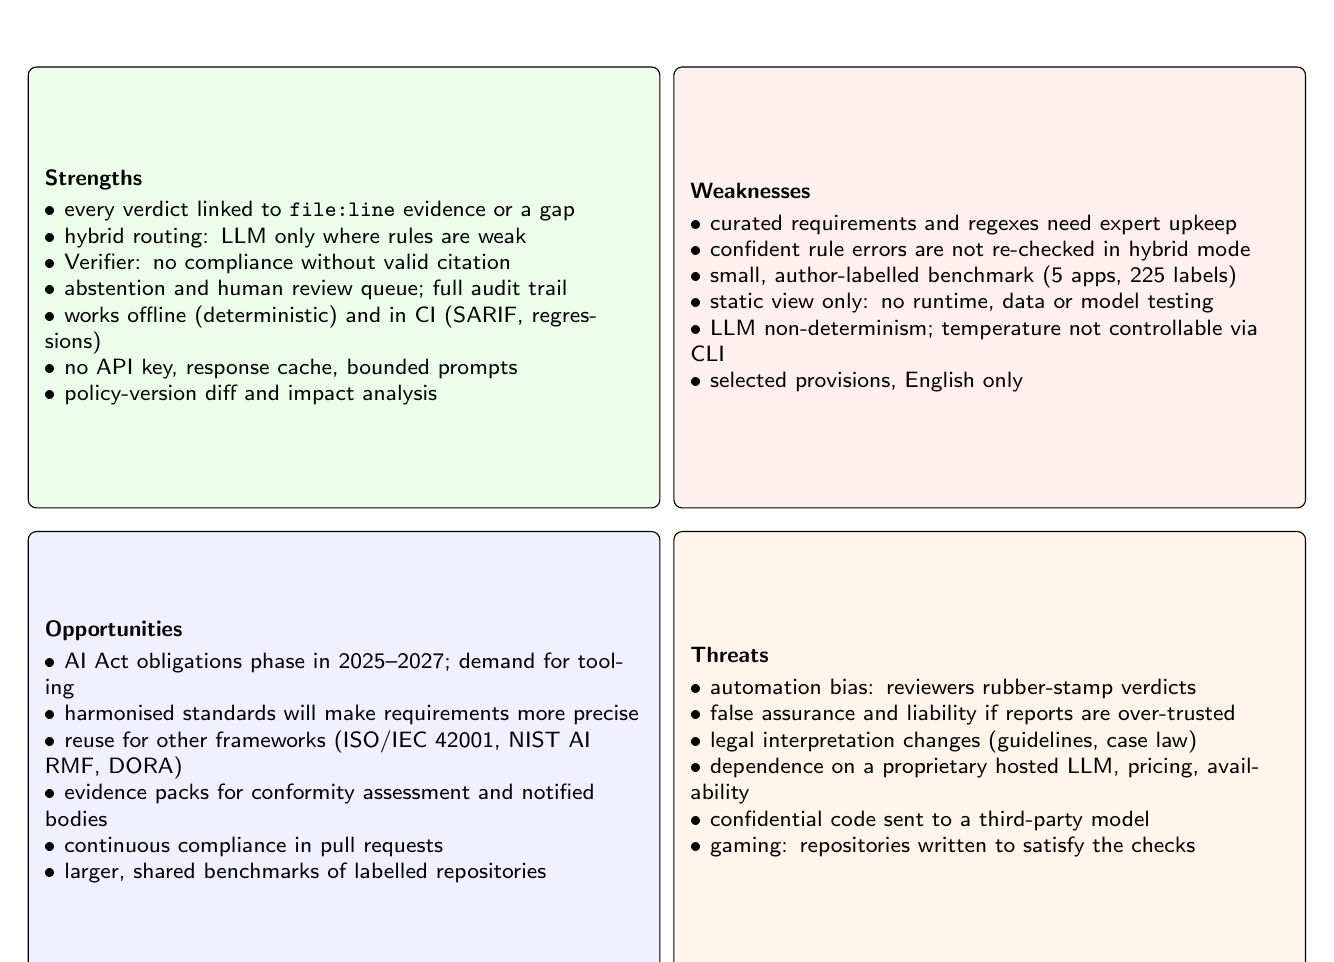
\begin{tikzpicture}[font=\sffamily\footnotesize,
  q/.style={draw, rounded corners=3pt, text width=7.6cm, minimum height=5.6cm, align=left, anchor=north west, inner sep=6pt}]
  \node[q, fill=green!8]  at (0,0)        {\textbf{Strengths}\\[2pt]
    \textbullet\ every verdict linked to \texttt{file:line} evidence or a gap\\
    \textbullet\ hybrid routing: LLM only where rules are weak\\
    \textbullet\ Verifier: no compliance without valid citation\\
    \textbullet\ abstention and human review queue; full audit trail\\
    \textbullet\ works offline (deterministic) and in CI (SARIF, regressions)\\
    \textbullet\ no API key, response cache, bounded prompts\\
    \textbullet\ policy-version diff and impact analysis};
  \node[q, fill=red!6]    at (8.2,0)      {\textbf{Weaknesses}\\[2pt]
    \textbullet\ curated requirements and regexes need expert upkeep\\
    \textbullet\ confident rule errors are not re-checked in hybrid mode\\
    \textbullet\ small, author-labelled benchmark (5 apps, 225 labels)\\
    \textbullet\ static view only: no runtime, data or model testing\\
    \textbullet\ LLM non-determinism; temperature not controllable via CLI\\
    \textbullet\ selected provisions, English only};
  \node[q, fill=blue!6]   at (0,-5.9)     {\textbf{Opportunities}\\[2pt]
    \textbullet\ AI Act obligations phase in 2025--2027; demand for tooling\\
    \textbullet\ harmonised standards will make requirements more precise\\
    \textbullet\ reuse for other frameworks (ISO/IEC 42001, NIST AI RMF, DORA)\\
    \textbullet\ evidence packs for conformity assessment and notified bodies\\
    \textbullet\ continuous compliance in pull requests\\
    \textbullet\ larger, shared benchmarks of labelled repositories};
  \node[q, fill=orange!8] at (8.2,-5.9)   {\textbf{Threats}\\[2pt]
    \textbullet\ automation bias: reviewers rubber-stamp verdicts\\
    \textbullet\ false assurance and liability if reports are over-trusted\\
    \textbullet\ legal interpretation changes (guidelines, case law)\\
    \textbullet\ dependence on a proprietary hosted LLM, pricing, availability\\
    \textbullet\ confidential code sent to a third-party model\\
    \textbullet\ gaming: repositories written to satisfy the checks};
\end{tikzpicture}
\caption{SWOT analysis of the Compliance-as-Code AI Auditor.}
\label{fig:swot}
\end{figure}

\paragraph{Mitigations.} Automation bias is countered by showing evidence before the verdict in the review sheet and by
requiring a justification for every override; vendor dependence by the backend protocol (any model behind
\texttt{complete\_json}) and the deterministic fallback; gaming by the LLM judge, which reads the whole context instead of
matching tokens, and by the decoy-style tests of the benchmark.

\chapter{Conclusions and future work}
\label{chapter:concl}

We framed the checking of an application repository against a regulation as grounded, selective classification:
every requirement receives a status, a confidence and citations, and the system may abstain in favour of a human. The
Compliance-as-Code AI Auditor implements this with a hybrid of deterministic policy-as-code checks and an LLM judge
(Claude via the Claude Code CLI in headless mode) constrained by retrieval, a strict citation contract, a Verifier and a
human-in-the-loop gate. It turns three policies (selected EU AI Act provisions, GDPR, an internal responsible-AI policy)
into 45 testable requirements and produces auditable reports in JSON, Markdown, SARIF and a web dashboard, with CI
regression gating and policy-version impact analysis.

On a benchmark of five hand-labelled AI applications (165 applicable labels), the main findings are:
\begin{itemize}[leftmargin=*]
  \item the hybrid mode is the most accurate (94.5\% accuracy, 86.6\% macro-F1), ahead of deterministic (82.4\%) and
        LLM-only (90.9\%);
  \item it needs 39\% fewer LLM calls than LLM-only, costs 41\% less and runs 45\% faster;
  \item it misses only 2 of 65 gaps, and all citations are valid;
  \item LLM-only mode is the most conservative (no false compliance), at the price of more false alarms.
\end{itemize}
Analysing the baseline errors improved accuracy by 3 (deterministic), 8 (hybrid) and 19 (LLM-only) points. The improvements were
comment-aware rules, graded rule confidence with a routing threshold chosen out-of-sample, and a rubric-aligned judge.
We recommend hybrid with Sonnet and $\tau=0.675$ as the default, LLM-only for high-stakes audits, and deterministic
mode for free, offline pre-commit checks.

\paragraph{Most important points.} (1) Rules and LLMs fail in complementary ways, so routing between them is worth more
than either alone; (2) the costliest auditor error, false compliance, can be controlled structurally (citations,
conflicts, abstention) rather than only statistically; (3) an auditor must be auditable: the record of who or what
decided each verdict, on which evidence, is as important as the verdict.

\paragraph{Future work.}
\begin{itemize}[leftmargin=*]
  \item \emph{Routing}: always route value-bearing checks (retention periods, amount thresholds) to the judge, which
        would remove the two remaining false compliances; learn the routing policy from review outcomes (active
        learning from the human queue).
  \item \emph{Requirements}: evaluate PolicyAnalyst-derived requirements against the curated ones; cover the full AI Act
        and harmonised standards; multilingual policies and repositories.
  \item \emph{Evidence}: dense or hybrid retrieval, cross-file reasoning (call graphs), runtime evidence (logs, metrics,
        model evaluations) in addition to static artefacts.
  \item \emph{Safety}: secret/PII redaction before prompting, local open-weight models for confidential code, calibration
        of the judge's confidence on review outcomes.
  \item \emph{Evaluation}: more and larger repositories labelled by independent annotators, with inter-annotator
        agreement.
\end{itemize}


\bibliographystyle{plainnat}
\bibliography{refs}

\end{document}
